\documentclass{article}
\usepackage[utf8]{inputenc}
\usepackage[top=2.5cm,bottom=2.5cm,right=2.5cm,left=2.5cm]{geometry}

\usepackage{graphics}
\usepackage{indentfirst,xspace}
\usepackage{graphicx,amssymb,dsfont,Sweave}
\usepackage[svgnames,usenames,dvipsnames,table]{xcolor}
\usepackage[toc,page]{appendix}
\usepackage{underscore}
\usepackage{amsmath,amsfonts,amsxtra,amsthm}
\usepackage{url}
\usepackage{pdfpages}
\usepackage[round]{natbib}
\usepackage{float}

%--------- Theorems commands
\newtheorem{theorem}{Theorem}[section]
\newtheorem{corollary}{Corollary}[theorem]
\newtheorem{lemma}[theorem]{Lemma}
\newtheorem*{remark}{Remark}

%----------------------------------------------------------------------------------
\definecolor{Red}{rgb}{0.5,0,0}
\usepackage[hyperfootnotes=true]{hyperref}
\hypersetup{
  colorlinks,
  citecolor=NavyBlue,
  linkcolor=MidnightBlue,
  urlcolor=Red
}

\usepackage{cleveref}

%\VignetteIndexEntry{GKF package examples}
%\VignettePackage{GKF}
%\VignetteKeyword{State space models}
%\VignetteKeyword{Kalman filter}
%\VignetteKeyword{nonlinear non-Gaussian models}\usepackage{ntheorem}


\newcommand{\R}{\texttt{R}\xspace}
\newcommand{\GKF}{\texttt{GKF}\xspace}

% mathematical notation
\DeclareMathOperator{\var}{var}
\DeclareMathOperator{\cov}{cov}
\DeclareMathOperator{\E}{\mathsf{E}}
\DeclareMathOperator{\Prob}{\mathsf{P}}

\newenvironment{comment}{%
  \begin{quote}\color{red}\begin{sffamily}}
 {\end{sffamily}\color{black}\end{quote}}


\begin{document}


% $

\title{\GKF Package Example (Version 1.6)}
\author{Tarak Kharrat and Georgi N. Boshnakov}
\maketitle


\section*{Introduction}

\GKF is an \R package for computations with state space models. It deals with the linear
Gaussian as well as the nonlinear non-Gaussian case. It is mostly written in \texttt{C++} and
relies fully on linear algebra subroutines contained in the Armadillo library
\citep{sanderson2010armadillo}.

This paper shows how \GKF can be used to fit general state space models and is by no means a
tutorial on state space models. We will explain how filtering and smoothing can be done, how
to estimate the parameters by maximum likelihood and how to sample (smoother) from the
(conditional) posterior distribution of the signal through univariate and multivariate
examples. We refer readers interested in a more theoretical treatement to
\citet{durbin2012time}. We do not restrict our treatment to the \GKF package but alternatives
using other \R packages (when it is possible) are presented. This approach has two
advantages: validate the computation done by \GKF and allow users to choose between the
different tools.

\begin{comment}
  We need here a review of what packages like FKF, dlm, KFAS do and don't do (and we do).

  Addition in March 2018: see also \citet{KFASjss2017}
\end{comment}

The remainder of this paper is structured as follows. In Section~\ref{sec:modelDef} we recall
the state space model, set the notation framework and show how to define such models with
\GKF using the case of a univariate auto-regressive moving average (ARMA) process. An example
of maximum likelihood estimation is presented in Section~\ref{sec:MLE}. Filtering and
smoothing are treated in Section~\ref{sec:FilterSmoothing} in the univariate and multivariate
case. Section~\ref{sec:SamplingSmoother} describes sampling (smoother) from the signal
posterior distribution which can be useful for estimation based on simulation techniques such
as importance sampling. An additional (multivariate) illustration is fully studied in
Section~\ref{sec:additional example}. A nonlinear non-Gaussian case is discussed in
Section~\ref{sec:nLnGaussian}. We conclude in Section~\ref{sec:CL}.

\section{The Model}
\label{sec:modelDef}

%%% A state space model consists of a transition equation and a measurement equation.
%%% The transition equation models the evolution of the state vector,
%%% $\alpha_t$, which in most applications is unobserved or partially observed.

Let $\{y_{t}\}$, $t=1,\dots,n$, be the $(d\times1)$ observed process.
For the observed process, $\{y_{t}\}$, we consider a general nonlinear non-Gausian model,
driven by a linear Markov state process.
In the case of the nonlinear non-Gaussian observation model we assume that the conditional
density of $y_{t}$, given the information up to time $t$, is a function of a $d \times 1$
signal vector $\theta_{t}$ and a vector of parameters $\psi$. We denote this density by
$p(y_{t}|\theta_{t};\psi)$ and write symbolically
\begin{equation}
  \label{eq:measurementH}
  y_{t} \sim p(y_{t}|\theta_{t};\psi)
  .
\end{equation}
The linear Gaussian observation model is usually specified by an
explicit equation for $y_{t}$:
\begin{equation}
  \begin{array}{rcl}
    y_{t}  = \theta_t + \epsilon_t,
    & \epsilon_t \sim \mathcal{N}(0,H_t),
    & t=1,\dots,n
    ,
  \end{array}
  \label{eq:measurement}
\end{equation}
where the $\epsilon_t$'s are independent and the variance matrices $H_t$ are fixed and known
or can partly depend on the vector parameter $\psi$.  The linear Gaussian observation model
can be viewed as a particular case of the general model, in which $p(y_{t}|\theta_{t};\psi)$
is the Gaussian density $\mathcal{N}(\theta_{t}, H_{t})$ and the variance matrices do not
depend on the past information.

In both cases, the signal is modelled as a linear transformation of a state vector
$\alpha_t$, i.e.
\begin{equation*} \label{eq:thetat}
  \theta_t = c_t + Z_t \alpha_t
  ,
\end{equation*}
where the intercept vector $c_t$ ($d \times 1$) and the factor matrix $Z_t$ ($d \times m$)
can also partialy depend on $\psi$.

For the state $\alpha_t$ we consider the linear Markov model with Gaussian innovations
defined by the following (transition) equation:
\begin{equation}
  \begin{array}{rccl}
    \alpha_{t+1}  =  d_t + T_t \alpha_t + \eta_t, & \eta_t \sim \mathcal{N}(0,Q_t),
    & t=1,\dots,n,
  \end{array}
  \label{eq:Transition}
\end{equation}
where $\alpha_t$ ($m \times 1$) is the state vector, $d_t$ ($m \times 1$) is the intercept,
$T_t$ ($m \times m$) is the factor
\textbf{(fixme: is this usual?  transition/state/system)}
matrix and $\eta_t$ ($m \times 1$) is the innovation (with ($m \times m$) variance matrix
$Q_t$) of the transition equation. The vector $d_t$ and matrices $T_t$ and $Q_t$ can partly
depend on the parameter vector $\psi$ and be partly fixed and known for $t=1,\dots, n$. The
matrix $Q_t$ is only required to be \textbf{positive semi-definite}. The initial state vector
$\alpha_{0}$ \textbf{(fixme: $\alpha_{1}$ or $\alpha_{0}$?)}
is normally distributed with mean $a$ and variance $P_{0}$. The innovations $\eta_t$ are
serially independent and are independent of the initial state vector for $t=1,\dots, n$.


% An example of this class will be discussed in Section~\ref{sec:nLnGaussian}.


The model specified by equations \eqref{eq:measurement}--\eqref{eq:Transition} is known also
as dynamic linear model (dlm).

The power of state space models comes from efficient recursive computations based on the above
equations. Nevertheless, in development and presentation of the methodology it is often easier
and more clear to work with the big matrices and vectors obtained by pooling together the
corresponding quantities for $t=1,\dots,n$.
To this end, define
the all times
observation vector ($dn \times 1$) $y=(y_1^\prime,\dots,y_n^\prime)^\prime$,
state vector ($ nm \times 1 $) $\alpha=(\alpha_1^\prime,\dots,\alpha_n^\prime)^\prime$,
signal vector ($dn \times 1$) $\theta=(\theta_1^\prime,\dots,\theta_n^\prime)^\prime$,
intercept vector ($dn \times 1$) $c=(c_1^\prime,\dots,c_n^\prime)^\prime$,
linear innovations vector ($dn \times 1$) $\epsilon = (\epsilon_{1}',\dots,\epsilon_{n}')$
and
matrices ($dn \times mn$) $\mathcal{Z}= \text{diag}(Z_1,\dots,Z_n)$
and ($dn \times dn$)  $H=\text{diag}(H_1,\dots,H_n)$.
For the all time signal we now have
\begin{equation*}
  \theta = c + \mathcal{Z} \alpha
  .
\end{equation*}
The linear observation equation can be written in matrix form as
\begin{equation}
  \begin{array}{rcl}
    y = \theta + \epsilon
      =  c + \mathcal{Z} \alpha + \epsilon
      , & \epsilon \sim \mathcal{N}(0,H) % , & H=\text{diag}(H_1,\dots,H_n)
    .
  \end{array}
  \label{eq:measurementVec}
\end{equation}

The state vector, $\alpha$, has a multivariate Gaussian distribution. More specifically,
$\alpha \sim \mathcal{N}(d,\Omega)$, where $d$ ($ nm \times 1 $) is given by
$d=T(a^\prime,d_1^\prime,\dots,d_{n-1}^\prime)^\prime $, $\Omega$ ($ nm \times nm $) by
$\Omega=T\text{diag}(P_1,Q_1,\dots,Q_{n-1})T^{\prime} $ and the $(i,j)$th block, $T_{ij}$, of
the lower block-triangular matrix $T$ (for $i,j=1,\dots,n$) is given by
\begin{equation}
T_{ij} = \begin{cases}
  0, & \mbox{if } i < j \\
  I, & \mbox{if } i=j \\
  T_{i-1} \times \dots \times Tj, & \mbox{if } i>j.
\end{cases}
\label{eq:Tij}
\end{equation}
The pattern of $T$ is important for computations, so we give it explicitly:
\begin{equation}
  T =
\begin{bmatrix}
  I      & 0   & 0 & 0  &  & 0 & 0 \\
  T_1    & I   & 0 & 0  &  & 0 & 0 \\
  T_2T_1 & T_2 & I & 0  &   & 0 & 0 \\
  T_3T_2T_1 & T_3T_2 & T_3 & I  &   & 0 & 0 \\
         &          &     &    &    \ddots &  & \vdots \\
  T_{n-2} \cdots T_1 & T_{n-2} \cdots T_2 & T_{n-2} \cdots T_3 & T_{n-2} \cdots T_4 & & I & 0 \\
  T_{n-1} \cdots T_1 & T_{n-1} \cdots T_2 & T_{n-1} \cdots T_3 & T_{n-1}  \cdots  T_4 & & T_{n-1} & I \\
\end{bmatrix}
\end{equation}
From the above it follows that the
all times signal vector  is multivariate normal, as well, and
\begin{equation}
  \begin{array}{rcl}
    \theta \sim \mathcal{N}(\mu,\Psi),
    & \mu=c+\mathcal{Z}d,
    & \Psi=\mathcal{Z} \Omega \mathcal{Z}^{\prime}
    .
  \end{array}
  \label{eq:SignalVec}
\end{equation}
\textbf{(fixme: give citations in this section)}



\section{Defining and manipulating state space models with GKF}

\subsection{Defining state space models with GKF}

\GKF accepts system variables prepared as matrices or arrays. Time-varying parameters are
given as arrays. Time-invariant parameters can also be specified as matrices which are
replicated as needed.
The correspondence between the variables in the equations in  Section~~\ref{sec:modelDef} and
the names in \GKF are given in the following table. For convenience we also give the
parameter names in package fkf.
\begin{center}
\begin{tabular}{l|ccccccccccc}
  parameter & $a_{0}$ & $P_{0}$ & $c_{t}$ & $d_{t}$ & $Z_{t}$ & $T_{t}$ & ?? & $Q_{t}$
  \\ \hline{}
  \GKF name & a0     & P0      & ct     & dt     & Zt     & Tt     & Ht & Qt
  \\
  fkf name  & a0     & P0      & ct     & dt     & Zt     & Tt     & GGt & HHt
\end{tabular}
\end{center}
The time series is a $(d\times n)$ matrix, where $d$ is the dimension of the time series.

A consistency check is done in each function (before computation starts) which can be
switched off by setting \verb@checkInputs@ to \verb@FALSE@. We advise users to keep
\verb@checkInputs@ \verb@TRUE@ unless the performance becomes crucial and correctness of the
arguments is ensured.


\subsubsection{Autoregressive moving average model}
An autoregressive moving average $\text{ARMA}(p, q)$ model is defined as
\begin{equation}
  \begin{array}{rccl}
    y_t & = & \phi_1 y_{t-1} + \dots + \phi_p y_{t-p} + \zeta_t + \theta_1 \zeta_{t-1} + \theta_q \zeta_{t-q}, & \zeta_t \sim \mathcal{N}(0,\sigma^2)
  \end{array}
  \label{eq:Armapq1}
\end{equation}
 with non-negative integers $p$ and $q$ and where $\zeta_t$ is a serially independent series of $ \mathcal{N}(0,\sigma^2)$ disturbances. This can be written in the form
\begin{equation}
  \begin{array}{rccl}
    y_t & = & \displaystyle \sum_{j=1}^r \phi_j y_{t-j} + \zeta_t + \sum_{j=1}^r \theta_j \zeta_{t-j}, & t=1,\dots,n
  \end{array}
  \label{eq:Armapq2}
\end{equation}
where $r = \max(p, q+1)$ and for which some coefficients are zero. These models can be
represented in state space form \citep[see][chap. 3.4]{durbin2012time}.

For example, consider the $\text{ARMA}(2, 1)$.
In this case $r=2$. There are various ways to put the model in state space form.
We set the state vector to $\alpha_{t} = (y_{t} , \phi_2 y_{t-1} + \theta_1 \zeta_{t})'$.
The associated transition equation is
\begin{equation*}
  \begin{pmatrix}
    y_{t+1}\\
    \phi_2 y_t + \theta_1 \zeta_{t+1}
  \end{pmatrix}
  =
  \begin{bmatrix}
    \phi_1 & 1 \\
    \phi_2 & 0
  \end{bmatrix}
  \begin{pmatrix}
    y_{t}\\
    \phi_2 y_{t-1} + \theta_1 \zeta_{t}
  \end{pmatrix}
  +
  \begin{pmatrix}
    1\\
    \theta_1
  \end{pmatrix}
  \zeta_{t+1}
  \label{eq:Arma21}
\end{equation*}
The measurement equation is given by $y_t = Z_t \alpha_t$, which implies that $\epsilon_t=0 $
(and hence $H_t=0$), $Z_t=[1 \ 0]$.  Note that $ \eta_t = \binom{1}{\theta_1}\zeta_{t+1} $
and hence $ Q_t= \sigma^2 \binom{1}{\theta_1} \binom{1}{\theta_1}^\prime$.

Here we use Example~1 from the demos in package FKF \citep{FKFpackage}, where the following
function to construct a state space representation from the four parameters of an
$\text{ARMA}(2, 1)$ model can be found:
\begin{Schunk}
\begin{Sinput}
> arma21ss <- function(ar1, ar2, ma1, sigma) {
+     Tt <- matrix(c(ar1, ar2, 1, 0), ncol = 2)
+     Zt <- matrix(c(1, 0), ncol = 2)
+     ct <- matrix(0)
+     dt <- matrix(0, nrow = 2)
+     GGt <- matrix(0)
+     H <- matrix(c(1, ma1), nrow = 2) * sigma
+     HHt <- H %*% t(H)
+     a0 <- c(0, 0)
+     P0 <- matrix(1e6, nrow = 2, ncol = 2)
+     list(a0 = a0, P0 = P0, ct = ct, dt = dt,
+          Zt = Zt, Tt = Tt, GGt = GGt, HHt = HHt)
+ }
\end{Sinput}
\end{Schunk}
For simplicity, the initial covariance matrix is set to a diffuse value. Note that the
usual convention is to set the diffuse initial matrix to a diagonal matrix, e.g.
\begin{Schunk}
\begin{Sinput}
> P0 <- diag(1e6, nrow = 2, ncol = 2)
\end{Sinput}
\end{Schunk}
but we keep the original function from FKF.

Here we simulate from an $\text{ARMA}(2,1)$ process. 
\begin{Schunk}
\begin{Sinput}
> ar1 <- 0.6
> ar2 <- 0.2
> ma1 <- -0.2
> sigma <- sqrt(0.2)
> n <- 1000
> a <- arima.sim(model = list(ar = c(ar1, ar2), ma = ma1), n = n,
+                innov = rnorm(n) * sigma)
\end{Sinput}
\end{Schunk}

This prepares the model and the time series for \GKF:
\begin{Schunk}
\begin{Sinput}
> sp <- arma21ss(ar1, ar2, ma1, sigma)
> yt <- rbind(a)
\end{Sinput}
\end{Schunk}
The time series is transformed to a matrix with one row, since this is a univariate time
series.

\begin{comment}
  G: Strictly speaking, for the unconditional log-likelihood we need the exact initial
  cov. matrix, unless we estimate $P_{0}$ along with the other param.
\end{comment}
We can compute, for example, the unconditional log-likelihood of the process and check the
result against the computation of the \texttt{FKF} package
\begin{Schunk}
\begin{Sinput}
> logLikikGKF <- FKF(a0 = sp$a0, P0 = sp$P0, dt = sp$dt, ct = sp$ct, Tt = sp$Tt,
+                    Zt = sp$Zt, Qt = sp$HHt, Ht = sp$GGt, yt = yt)$logLik
\end{Sinput}
\end{Schunk}
\textbf{Note on 2018-03-29:} We load an object created by "fkf" since the package FKF has
been archived recently on CRAN, so may not be available. If you have it installed, run the
commented out command below to create it:
\begin{Schunk}
\begin{Sinput}
> ## logLikfkf <- FKF::fkf(a0 = sp$a0, P0 = sp$P0, dt = sp$dt, ct = sp$ct, Tt = sp$Tt,
> ##                       Zt = sp$Zt, HHt = sp$HHt, GGt = sp$GGt, yt = yt)$logLik
> logLikfkf <- readRDS("logLikfkf.rds")
\end{Sinput}
\end{Schunk}
Note the notation differences for the innovation variance and perturbation variance between
\verb@FKF@ and \GKF.

The log-likelihoods computed by GKF and FKF are the same:
\begin{Schunk}
\begin{Sinput}
> all.equal(logLikikGKF, logLikfkf)
\end{Sinput}
\begin{Soutput}
[1] TRUE
\end{Soutput}
\end{Schunk}



\section{Maximum Likelihood Estimation}
\label{sec:MLE}

As discussed in Section~\ref{sec:modelDef}, the system variables can partly depend on some
unknown vector $\psi$ that needs to be estimated. One way to do that is by maximum
likelihood. We illustrated in the previous section that \GKF returns the log-likelihood
$p(y|\psi)$ when the function \texttt{FKF} is called. We can use it as the objective function
of a desired optimization routine after providing some initial guess to obtain estimates of
$\psi$. We illustrate this procedure for the local level model and the Nile river dataset.

\subsection{The local level model}
The local level model is another example of univariate dynamic linear model. It is described
by the equations
\begin{equation*}
   \begin{array}{rccl}
     y_t & = & \alpha_t + \epsilon_t &  \epsilon_t \sim  \mathcal{N}(0,\sigma_\epsilon^2) \\
     \alpha_{t+1} & = & \alpha_t + \eta_t &  \eta_t \sim  \mathcal{N}(0,\sigma_\eta^2) \\
    \end{array}
  \label{eq:measurementNLNG}
\end{equation*}
for $t = 1,\dots, n $, where the $\epsilon_t$’s and $\zeta_t$’s are all mutually independent
and are independent of $\alpha_1$. Although it has a simple form, this model is not an
artificial special case and indeed it provides the basis for the analysis of important real
problems in practical time series analysis.


\subsection{The Nile River dataset}
The Nile River dataset is shipped with \R and represents the measurements of the annual flow
of the river at Ashwan betwenn 1871 and 1970 (100 observation). The local level model with
unknown measurement and transition variances is knowm to describe the data reasonably
well. The following peace of code show how to fit this model to the data using \verb@optim@
to minimize the inverse of the log-likelihood. We also assume that some observation are
missing to illustrate how \GKF treats \verb@NA@ (missing values are respresented by
\verb@NA@)
\begin{Schunk}
\begin{Sinput}
> y <- c(Nile)
> y[c(3, 10)] <- NA # NA values can be handled
> dt <- ct <- matrix(0)
> Zt <- Tt <- matrix(1)
> a0 <- y[1] # Estimation of the first year flow
> P0 <- matrix(100) # Variance of a0
> yt <- rbind(y)
> fit.GKF <- optim(c(Qt = var(y, na.rm = TRUE) * .5,
+                    Ht = var(y, na.rm = TRUE) * .5 ),
+                  fn = function(par, ...)
+                      -FKF(Qt = matrix(par[1]),
+                           Ht = matrix(par[2]), ...)$logLik,
+                  yt = yt, a0 = a0, P0 = P0, dt = dt, ct = ct,
+                  Zt = Zt, Tt = Tt, checkInputs = TRUE)
> Qt <- matrix(fit.GKF$par[1])
> Ht <- matrix(fit.GKF$par[2])
> GKF.obj <- FKF(a0 = a0, P0 = P0, dt = dt, ct = ct, Tt = Tt, Zt = Zt,
+                Qt = Qt, Ht = Ht, yt =  yt)
> fit.stats <- StructTS(y, type = "level")
\end{Sinput}
\end{Schunk}

% $

\section{Filtering and Smoothing with \GKF}
\label{sec:FilterSmoothing}

In the linear Gaussian case, when all the system variables are known, the joint distribution
of states and observations is Gaussian. Hence, it is fairly easy to derive conditional
distributions of states, signals, disturbances, innovations or future observations
conditional on the observed data. Such operations are called filtering, smoothing and
forecasting (\textbf{TODO:} not implemented by \GKF yet), respectively and are discussed in
the following sections for the signal $\theta_t$ or state $\alpha_t,t=1,\dots,n$ vectors
depending on the context. Note that given the linear transformation defining the signal from
the state, when the Gaussian assumption applies, it is straightforward to obtain the
conditional (on the data) mean and variance of the signal knowing the mean and variance of
the state.

\subsection{Filtering}

The filtering distribution of the state at time $t$ is the conditional distribution of
$\alpha_t$ given the observed data up to time $t$, i.e,
$Y_t=(y_1^\prime,\dots,y_t^\prime)^\prime$. Given that this distribution is Gaussian,
filtering reduces to the computation of $a_{t|t}=\E[\alpha_t|Y_t]$ (the mode of
$p(\alpha_t|y_1,\dots,y_t)$) and $P_{t|t}=\var[\alpha_t|Y_t]$, which is achieved by a
(forward) recursive procedure, based on the celebrated Kalman filter algorithm or extensions
thereof.  The main ingredient of the Kalman filter derivation is recalled in
Appendix~\ref{sec:MultiVNormal} and the resulting equations are collected in
Equation~\eqref{eq:KFForward} although in a different context. Readers interested in the
details of the derivation are referred to \citet[chap. 4]{durbin2012time}.

We illustrate the filtering for the local level model described earlier and for a
multivariate example inspired from \citet[chap. 3.3.2]{petris2009dynamic}.

\subsubsection{Filtering for the Local Level Model}

Consider again the model fitted to the Nile river data. Taking the estimated parameters as
known, filtering was computed (by a call to \texttt{FKF}) and results stored in
\texttt{GKF.obj} (following standard notations, filtered mean is named \texttt{att} and the
associated variance \texttt{Ptt}).  Figure~\ref{fig:nileFilter}
(page~\pageref{fig:nileFilter}) shows flow data together with fitted local levels
\begin{Schunk}
\begin{Sinput}
> plot(y, main = "Nile flow", col = "brown")
> lines(GKF.obj$att[1, ], type = "o", pch = 20, col = "blue")
> legend("top", c("Nile flow data", "Local level (GKF)"),
+        col = c("brown", "blue"), lty = 1)
\end{Sinput}
\end{Schunk}
\begin{figure}[htbp]
  \centering
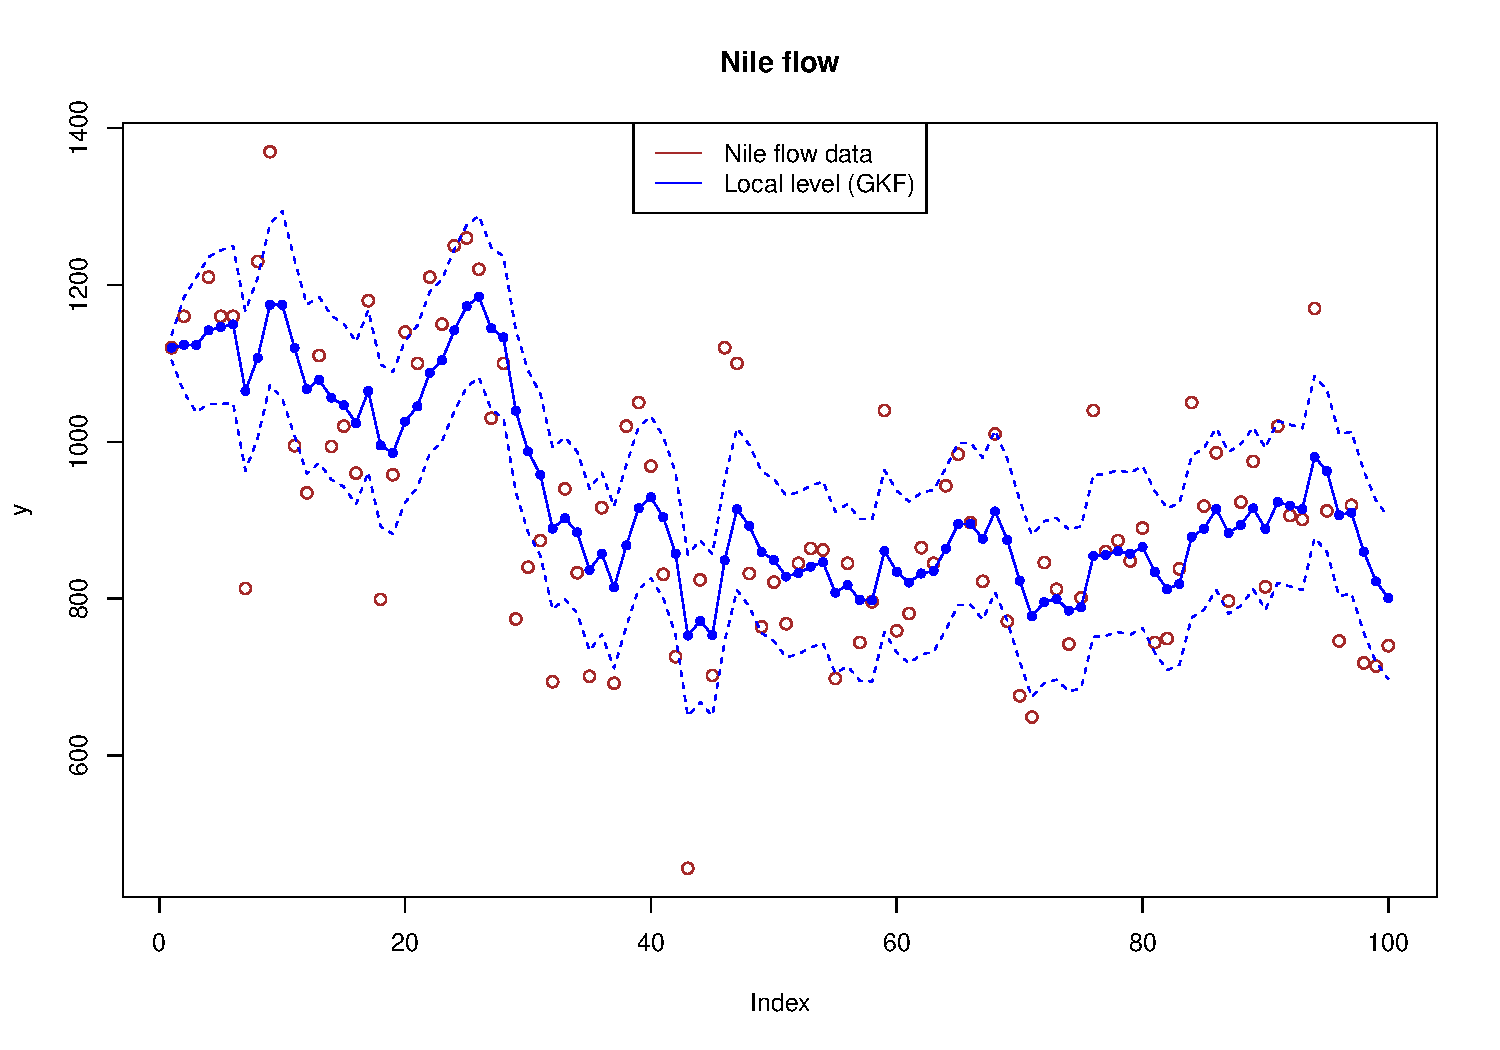
\includegraphics{vignette-011}
  \caption{Nile data with filtered level}
  \label{fig:nileFilter}
\end{figure}

We can also compute 95\% confidence intervals for the filtering estimate as follows:
\begin{Schunk}
\begin{Sinput}
> v <- as.numeric(GKF.obj$Ptt)
> pl <- GKF.obj$att[1, ] + qnorm(0.05, sd = sqrt(v))
> pu <- GKF.obj$att[1, ] + qnorm(0.95, sd = sqrt(v))
> lines(pl, lty = 2, col = "blue")
> lines(pu, lty = 2, col = "blue")
\end{Sinput}
\end{Schunk}

In addition to filtering means and variances (of the state), and the log-likelihood of the
conditional data, \texttt{FKF} returns some other quantities computed by the Kalman filter
that will be used for the smoothing and sampling. See \GKF documentation for more details.

\subsubsection{Multivariate Linear Growth Model}

The multivariate model considered here is obtained by assuming that the vector of observation
$y_t=(y_{1,t},\dots,y_{d,t})$ can by seen as $d$ independent series and study them
(independently) by specifying a univariate model for each of them. For example, each series
will have a state vector with a level and a slope component and a diagonal variance
matrix. This means that the evolution of the level and slope is governed by independent
random inputs and suggests describing the joint evolution of the state vectors by grouping
together all the levels and then all the slopes in an overall state vector
$\alpha_t = (\mu_{1,t},\dots, \mu_{d,t}, \beta_{1,t},\dots, \beta_{d,t})^{\prime}$. The
system error of the dynamics of this common state vector will then be characterized by a
block-diagonal variance matrix having a first $d \times d$ block accounting for the
correlation among levels and a second $d \times d$ block accounting for the correlation among
slopes. To be specific, suppose one has $d = 2$ series. Then
$\alpha_t = (\mu_{1,t}, \mu_{2,t}, \beta_{1,t}, \beta_{2,t})^{\prime} $ and the system
equation is
\begin{equation}
  \begin{pmatrix}
    \mu_{1,t+1}\\
    \mu_{2,t+1} \\
    \beta_{1,t+1}\\
    \beta_{2,t+1}
  \end{pmatrix}
  =
  \begin{bmatrix}
    1 & 0 & 1 & 0 \\
    0 & 1 & 0 & 1 \\
    0 & 0 & 1 & 0 \\
    0 & 0 & 0 & 1
  \end{bmatrix}
  \begin{pmatrix}
    \mu_{1,t}\\
    \mu_{2,t} \\
    \beta_{1,t}\\
    \beta_{2,t}
  \end{pmatrix}
  +
  \begin{pmatrix}
    \eta_{1,t}\\
    \eta_{2,t}\\
    \eta_{3,t}\\
    \eta_{4,t}
  \end{pmatrix}
  \label{eq:LinearGrowthState}
\end{equation}
where $(\eta_{1,t},\eta_{2,t},\eta_{3,t},\eta_{4,t})^{\prime} \sim \mathcal{N}(0,Q)$ and
\begin{equation*}
  Q = \left[\begin{array}{c|c}
              Q_{\mu} & 0 \\ \hline
              0 & Q_{\beta}
            \end{array}\right]
  ,
\end{equation*}
while the measurement equation is given by
% \begin{equation}
%   \begin{array}{rccc}
%     \begin{pmatrix}
%       y_{1,t}\\
%       y_{2,t}
%     \end{pmatrix}
%     & = &
%     \begin{bmatrix}
%       1 & 0 & 0 & 0 \\
%       0 & 1 & 0 & 0
%     \end{bmatrix}
%     \alpha_t + &
%     \begin{pmatrix}
%       \epsilon_{1,t}\\
%       \epsilon_{2,t}
%     \end{pmatrix}
%   \end{array}
%   \label{eq:LinearGrowthObs}
% \end{equation}
\begin{equation}
  \begin{pmatrix}
    y_{1,t}\\
    y_{2,t}
  \end{pmatrix}
  =
  \begin{bmatrix}
    1 & 0 & 0 & 0 \\
    0 & 1 & 0 & 0
  \end{bmatrix}
  \alpha_t +
  \begin{pmatrix}
    \epsilon_{1,t}\\
    \epsilon_{2,t}
  \end{pmatrix}
  ,
  \label{eq:LinearGrowthObs}
\end{equation}
with $(\epsilon_{1,t},\epsilon_{2,t})^\prime  \sim \mathcal{N}(0,H)$, where $H$ is allowed to be non-diagonal.

In order to illustrate the previous example, we use the data described in
\citet[chap. 3.3.2]{petris2009dynamic} and representing the annual investment in Denmark and
Spain from 1960 to 2000. This dataset was collected from \citet{petris2009dynamic} book
website \footnote{\url{http://definetti.uark.edu/~gpetris/dlm/}} and is shipped with the \GKF
package.

For this model we compare results from packages \texttt{dlm} (\cite{petris2010dlm}) and
\GKF. We start by loading the data:
\begin{Schunk}
\begin{Sinput}
> data(GKF_data)
> invest <- GKF.data$invest
\end{Sinput}
\end{Schunk}
After that, we set up the model in a '\texttt{dlm}' fashion
\begin{Schunk}
\begin{Sinput}
> library(dlm)
> mod <- dlm::dlmModPoly(2)
> mod$FF <- mod$FF %x% diag(2)
> mod$GG <- mod$GG %x% diag(2)
> W1 <- matrix(c(0.5, 0, 0, 0.5), 2, 2)
> W2 <- diag(c(49, 437266))
> W2[1, 2] <- W2[2, 1] <- 155
> mod$W <- bdiag(W1, W2)
> V <- diag(c(72, 14353))
> V[1, 2] <- V[2, 1] <- 1018
> mod$V <- V
> mod$m0 <- rep(0, 4)
> mod$C0 <- diag(4) * 1e4
\end{Sinput}
\end{Schunk}
The filtering in \texttt{dlm} is simply made by a call to the \texttt{dlmFilter} function,
which only requires the data and the model object. After some minor transformation, we can
easly obtain the filtered signal:
\begin{Schunk}
\begin{Sinput}
> filtered <- dlm::dlmFilter(invest, mod)
> alpha.filtered <- dlm::dropFirst(filtered$m)
> theta.filtered.dlm <- t(mod$FF %*% t(alpha.filtered))
\end{Sinput}
\end{Schunk}
The system object used by package \GKF is deduced from the \texttt{dlm} object as follows:
\begin{Schunk}
\begin{Sinput}
> a0 = mod$m0
> P0 = mod$C0
> dt = rep(0, 4)
> ct = rep(0, 2)
> Tt = mod$GG
> Zt = mod$FF
> Qt = mod$W
> Ht = mod$V
> yt = t(as.matrix(invest))
\end{Sinput}
\end{Schunk}
Filtering is done as before in \GKF by a call to \verb@FKF@. We decided to set
\verb@checkInputs@ to \verb@TRUE@ to replicate the system object accordingly, if needed.
\begin{Schunk}
\begin{Sinput}
> kf.GKF <- FKF(a0 = a0, P0 = P0, dt = dt, ct = ct, Tt = Tt, Zt = Zt, Qt = Qt,
+               Ht = Ht, yt = yt, checkInputs = TRUE)
> theta.filtered.GKF <- Zt %*% kf.GKF$att
\end{Sinput}
\end{Schunk}
Figure~\ref{fig:LGFilter} (page~\pageref{fig:LGFilter}) shows Denmark annual investment data
together with filtered signal values from \texttt{dlm} and \GKF. We notice that both graphs
agree except in the initial starting points due to the Bayesian approach adopted by
\texttt{dlm}, i.e, the effect of the prior distribution disapears after some time.
\begin{Schunk}
\begin{Sinput}
> i = 1
> plot(yt[i,],main = "Annual Denmark investments",col = "brown",xlab = NA, ylab = NA)
> lines(theta.filtered.dlm[,i],type = "l",lty = 6,pch = 20, col = "green")
> lines(theta.filtered.GKF[i,],type = "o",pch = 20, col = "blue")
\end{Sinput}
\end{Schunk}
\begin{figure}[htbp]
  \centering
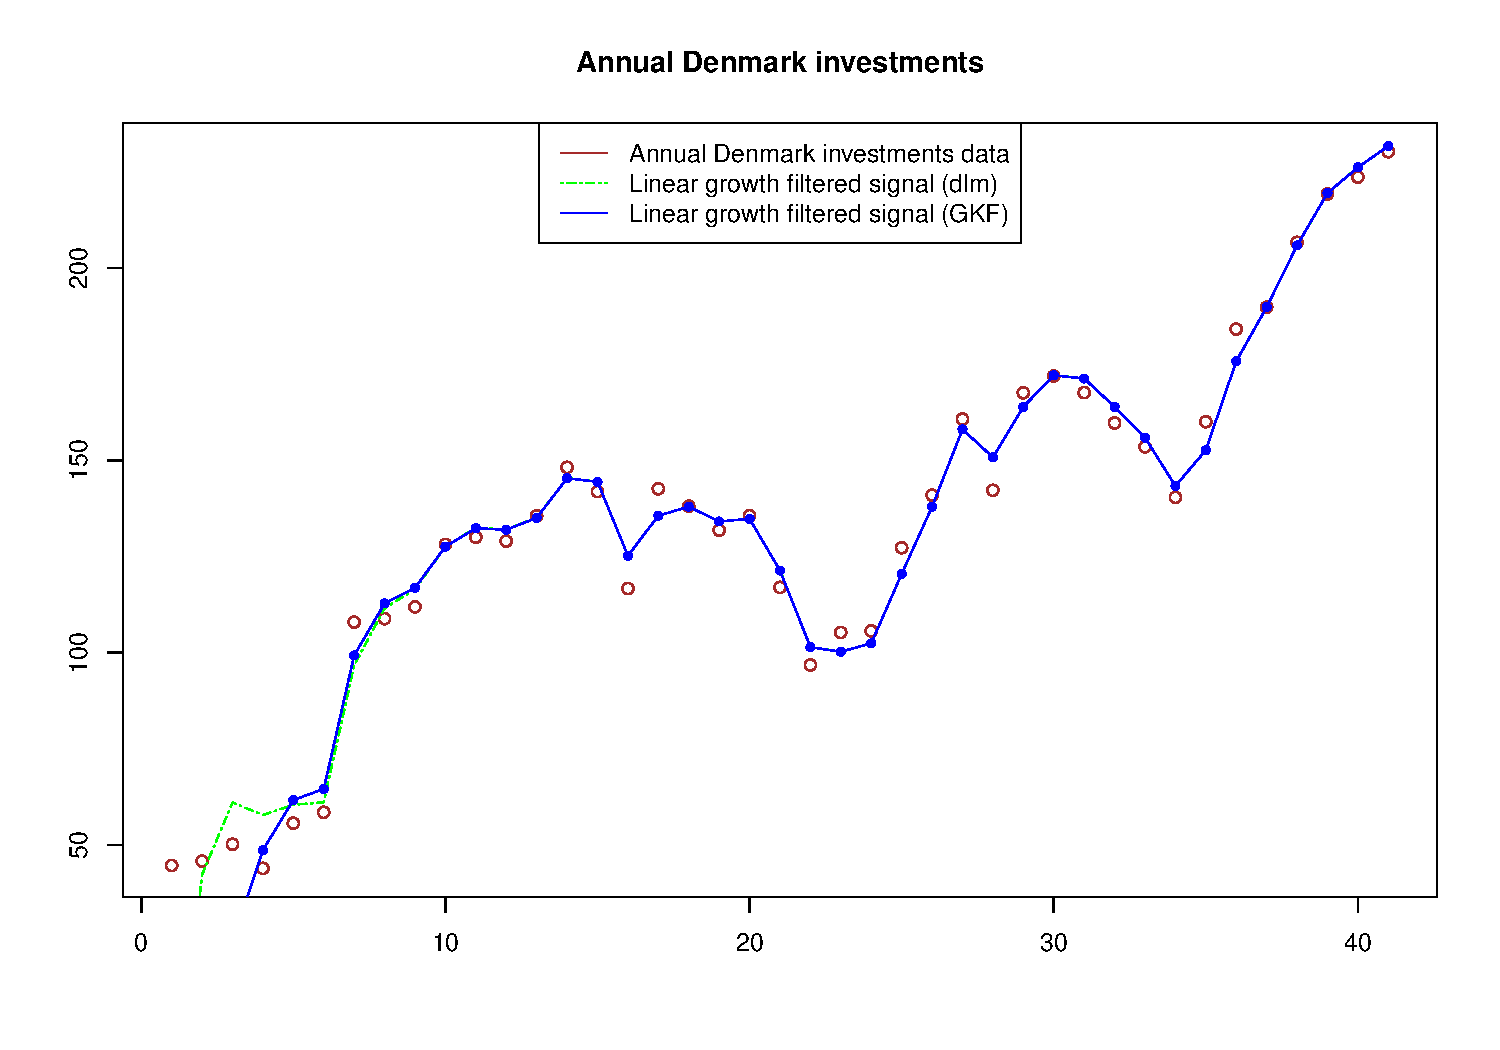
\includegraphics{vignette-019}
\caption{Denmark investment with filtered signal from \texttt{dlm} and \GKF}
\label{fig:LGFilter}
\end{figure}

\subsection{Smoothing}

The Smoothing distribution at time $t$ is the conditional distribution of $\alpha_t$ (state
smoothing) or $\theta_t$(signal smoothing) given the entire observed data i.e,
$y=(y_1^\prime,\dots,y_n^\prime)^\prime$. This distribution is also Gaussian, and its
characteristic elements can be computed by a (forward) recursive algorithm
\citep[see][chap. 4.5.3]{durbin2012time}. Note that \GKF only computes signal smoothing i.e,
$\hat{\theta}=\E[\theta_t|y]$ (the mode of $p(\theta_t|y)$) and $\var[\theta_t|y]$ by
adapting the disturbance smoothing recursions using the fact that
$\theta_t = y_t - \epsilon_t$ (hence $\hat{\theta}=y_t-\hat{\epsilon}$) and
$\var(\theta_t |y) = \var(\epsilon_t |y)$. The smoothed state can be easily obtained by
applying the appropriate linear transformation. Again, the technical result recalled in
\textit{Lemma 1}, Appendix~\ref{sec:MultiVNormal} is the main ingredient of the derivation.

We illustrate now how to obtain the smoothed signal for the (multivariate) linear growth
example discussed earlier using \GKF.  Figure~\ref{fig:LGSmooth}
(page~\pageref{fig:LGSmooth}) compares Spain annual investment data with filtered and
smoothed signal values.
\begin{figure}[htbp]
  \centering
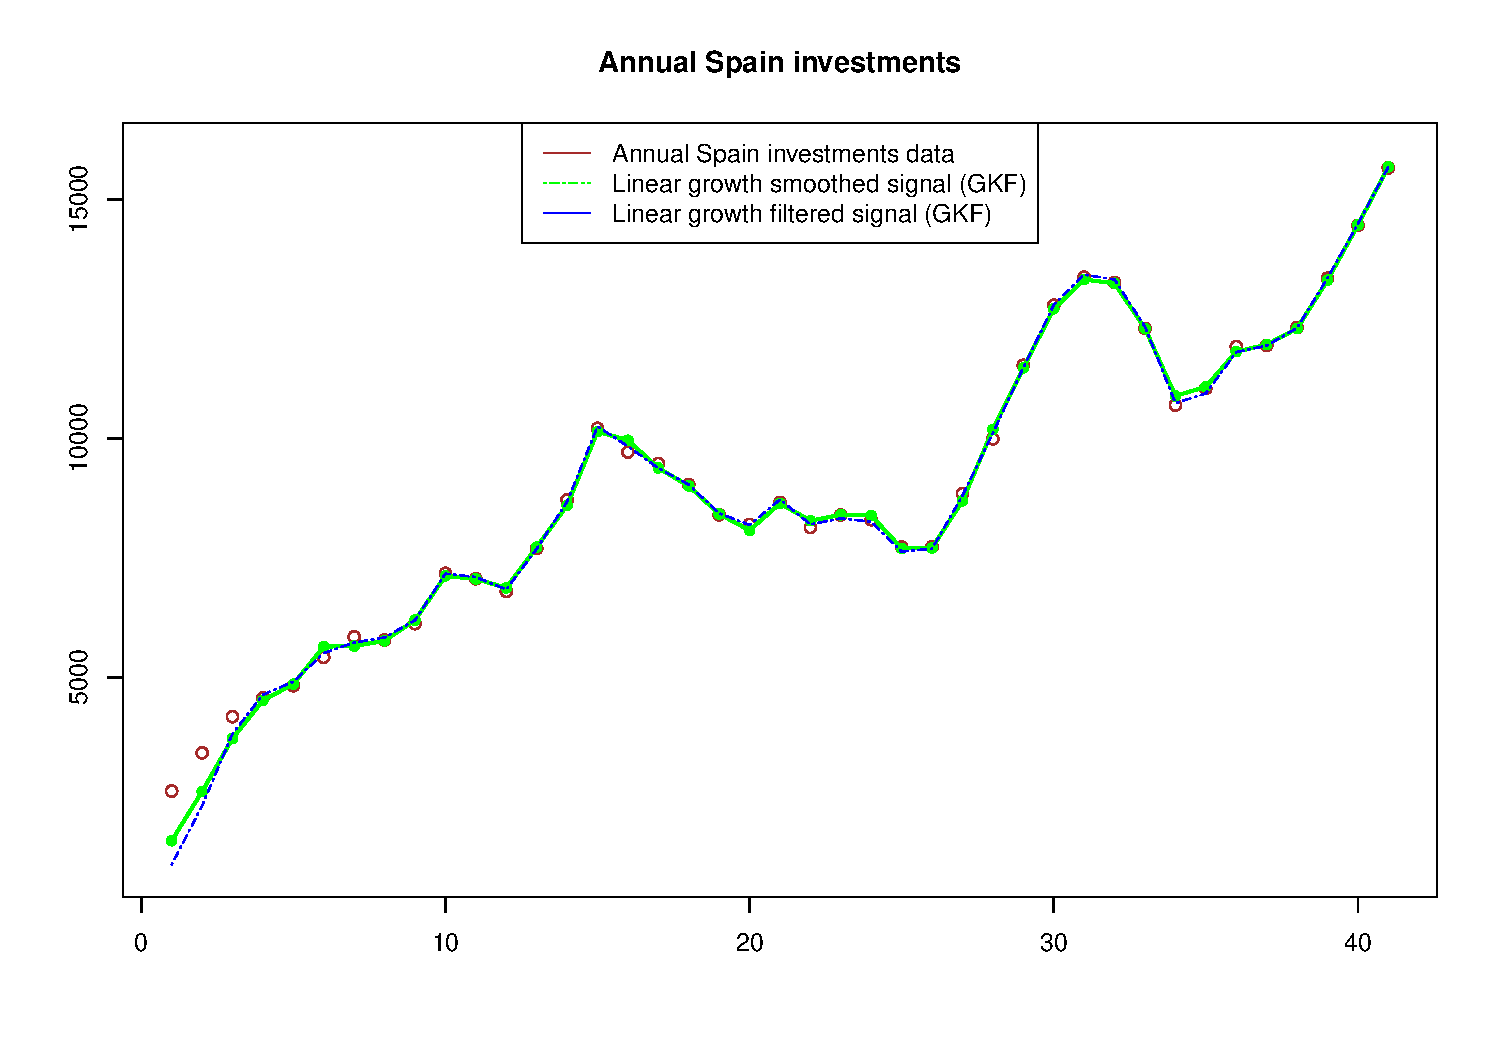
\includegraphics{vignette-020}
\caption{Spain investment with filtered and smoothed signal from \GKF}
\label{fig:LGSmooth}
\end{figure}

We notice a small difference at the first time points which disapears quickly at the end of
the observation window as higlighted by the following result:
\begin{Schunk}
\begin{Sinput}
> i = 2
> mat <- matrix(t(rbind(theta.smoothed.GKF[i, ], theta.filtered.GKF[i, ])), ncol = 2)
> colnames(mat) <- c("Smoothed", "Filtered")
> head(mat)
\end{Sinput}
\begin{Soutput}
     Smoothed Filtered
[1,] 1577.616 1077.298
[2,] 2606.264 2306.147
[3,] 3717.433 3817.201
[4,] 4516.029 4632.766
[5,] 4855.204 4906.939
[6,] 5641.648 5503.007
\end{Soutput}
\begin{Sinput}
> tail(mat)
\end{Sinput}
\begin{Soutput}
      Smoothed Filtered
[36,] 11814.23 11804.01
[37,] 11960.81 11941.68
[38,] 12299.36 12309.66
[39,] 13309.56 13356.06
[40,] 14466.83 14490.67
[41,] 15681.27 15681.27
\end{Soutput}
\end{Schunk}

\section{Sampling Smoother with \GKF}
\label{sec:SamplingSmoother}

In many simulation based techniques such as importance sampling or Markov Chain Monte Carlo
(MCMC), it is imperative to be able to sample from the state/signal (or the
disturbance/innovation) given the observed data that is for example drawing a sample
$\theta=(\theta_1^\prime,\dots,\theta_n^\prime)^{\prime} $ given
$y=(y_1^\prime,\dots,y_n^\prime)^\prime $. The first algorithms for the linear Gaussian model
has been suggested as early as 1994 by \citet{fruhwirth1994data} followed by
\citet{de1995simulation}. A simpler and computationally more efficient algorithm inspired
from the last cited paper was suggested by \citet{durbin2002simple} and recalled in
\citet[chap. 4.9]{durbin2012time}. This last technique also known as simulation smoothing by
mean corrections is the one implemented in \GKF. Note that only simulation smoother from the
signal conditional distribution is available in \GKF version 1.6.

An other family of simulation based algorithms known as Forward Filtering Backward Sampling
(FFBS) has been developed independently by \citet{carter1994gibbs} and
\citet{shephard1994partial}. The algorithm consists essentially in a simulation version of
the Kalman smoother. This alternative was implemented in \texttt{dlm}.

Before showing how to sample from the signal posterior distribution, it is interesting to get
a sense of the difference between conditional and unconditional sampling. We will use the
Nile river data to illustrate this point.

We first start by simulating unconditionally on the data using the state equation
(signal=state in the local level model)
\begin{Schunk}
\begin{Sinput}
> set.seed <- 1
> n <- length(yt)
> Nile.theta.uncond <- yt[1]
> for (i in 2:n) Nile.theta.uncond[i] <- Nile.theta.uncond[i-1] + rnorm(1,0,sqrt(Qt))
\end{Sinput}
\end{Schunk}
Then we use \GKF functions to produce and sample from the signal posterior distribution.
\begin{Schunk}
\begin{Sinput}
> Nile.theta.Smooth <- GaussianSignalSmoothing(
+     a0 = a0, P0 = P0, dt = dt, ct = ct, Tt = Tt, Zt = Zt, Ht = Ht, Qt = Qt, yt = yt
+               )$theta
> Nile.theta.cond <- GaussianthetaSampling(
+     a0 = a0, P0 = P0, dt = dt, ct = ct, Tt = Tt, Zt = Zt, Ht = Ht, Qt = Qt, yt = yt,
+          M = 1)$theta
\end{Sinput}
\end{Schunk}
Figure~\ref{fig:DiffSample} (page~\pageref{fig:DiffSample}) shows how bad the unconditional
sample describes the data. On the other hand, the simulated sample provides a fair view.
\begin{figure}[htbp]
  \centering
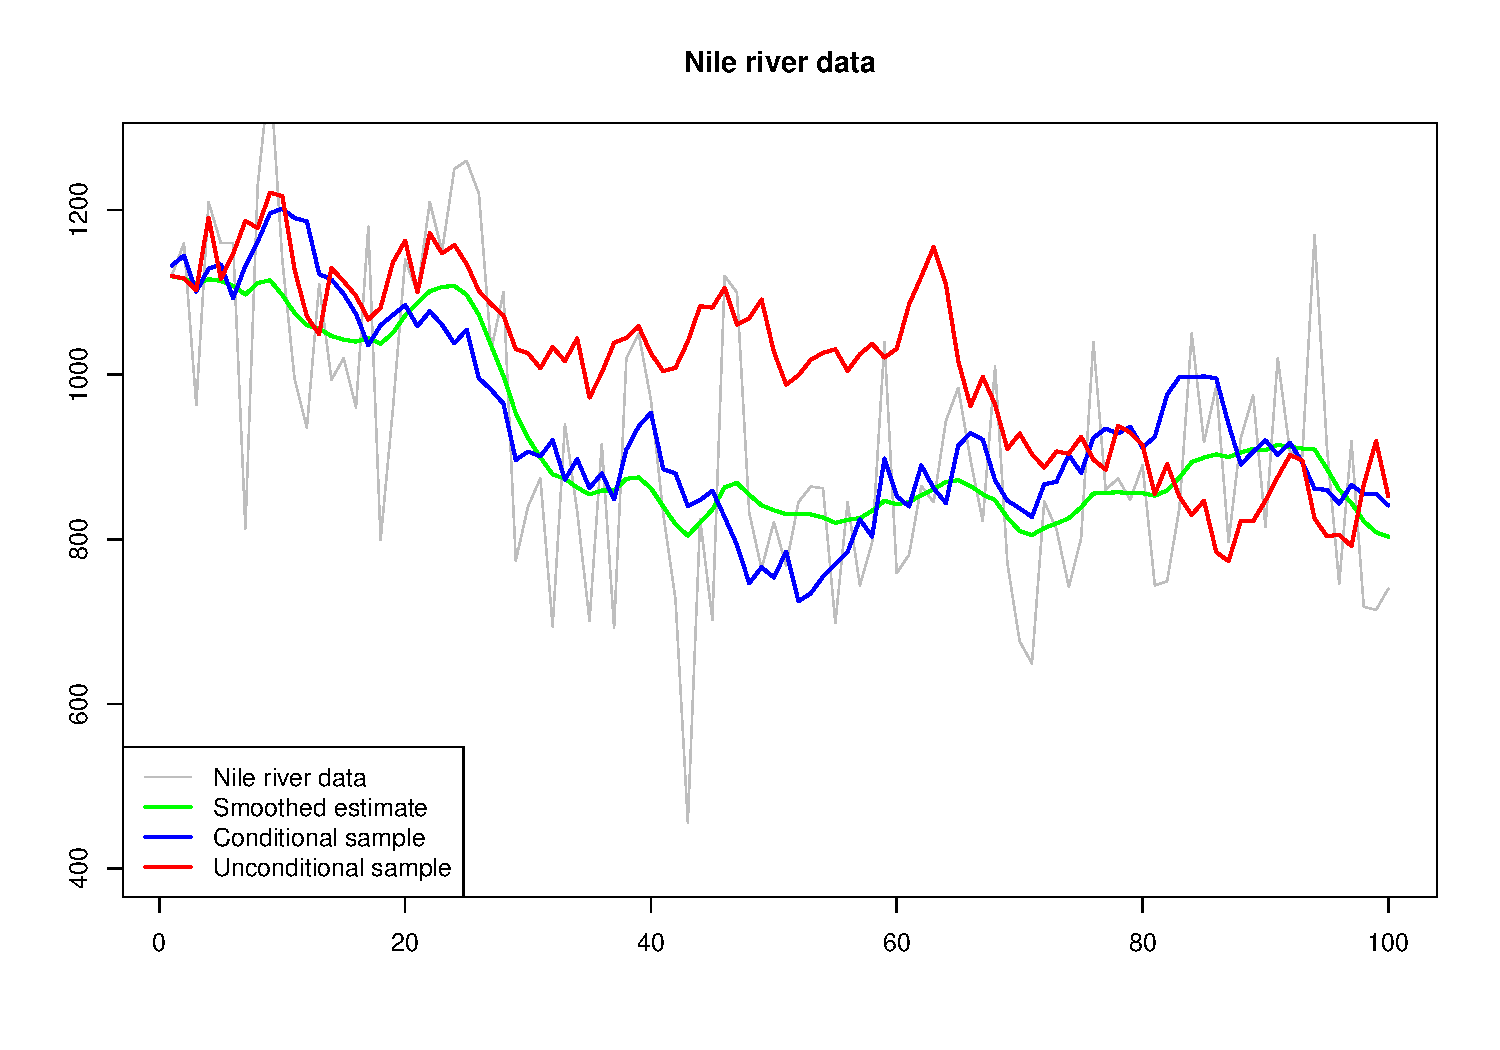
\includegraphics{vignette-025}
\caption{Comparison of the conditional and unconditional signal vector simulated sample.}
\label{fig:DiffSample}
\end{figure}

We briefly describe now the main ideas behind the simulation smoothing by mean
corrections. First, note that if one has a sample from the posterior disturbance
$\tilde{\epsilon} =(\epsilon_1,\dots,\epsilon_n)^\prime$ then a sample from the posterior
signal is simply obtained by $\tilde{\theta} = y - \epsilon $. The algorithm to simulate from
the posterior disturbance and innovation can be done in three major steps as follows:
\begin{itemize}
\item Define $\omega =(\epsilon^\prime,\eta^\prime)^\prime$. One starts by drawing a sample
  $\omega^+$ from $p(\omega)$ where $p(\omega) \sim \mathcal{N}(0,\Omega)$,
  $\Omega=\text{diag}(H_1,\dots,H_n,Q_1,\dots,Q_n).$ This sampe is then used to generate a
  sample $y^+$ from the observation by means of a recursive application of the measurement
  and transition equations \eqref{eq:measurement} and \eqref{eq:Transition}, where the
  recursion is initialized by the draw $\alpha_1^+ \sim \mathcal (a_1,P_1)$.

\item Use the Kalman filter forward recursion together with the smoothing backward recursion
  to compute $\hat{\omega}=(\hat{\epsilon}^\prime,\hat{\eta}^\prime)^\prime =\E[\omega|y]$
  and
  $\hat{\omega}^+=(\hat{\epsilon}^{+\prime},\hat{\eta}^{+\prime})^\prime =\E[\omega^+|y^+]$.

\item take the sample $\tilde{\omega}=\hat{\omega}-\hat{\omega}^+ + \omega^+$.

\end{itemize}

Finally we show how to sample from \GKF and \texttt{dlm}. \GKF provides the function
\texttt{GaussianthetaSampling} which allows to sample \texttt{M} times from the posterior
signal distribution. It requires the system objects as usual plus some optional inputs such
as the number of samples. We use the linear growth model to show its use.
\begin{Schunk}
\begin{Sinput}
> data(GKF_data)
> invest <- GKF.data$invest
> mod <- dlm::dlmModPoly(2)
> mod$FF <- mod$FF %x% diag(2)
> mod$GG <- mod$GG %x% diag(2)
> W1 <- matrix(c(500,0,0,500), 2, 2)
> W2 <- diag(c(49, 437266))
> W2[1, 2] <- W2[2, 1] <- 155
> mod$W <- bdiag(W1, W2)
> V <- diag(c(72, 14353))
> V[1, 2] <- V[2, 1] <- 1018
> mod$V <- V
> mod$m0 <- rep(0, 4)
> mod$C0 <- diag(4) * 1e4
> ## Rcpp
> a0 = mod$m0; P0 = mod$C0; dt = rep(0, 4); ct = rep(0, 2)
> Tt = mod$GG; Zt = mod$FF; Qt = mod$W; Ht = mod$V
> yt = t(as.matrix(invest))
\end{Sinput}
\end{Schunk}
\begin{figure}[htbp]
  \centering
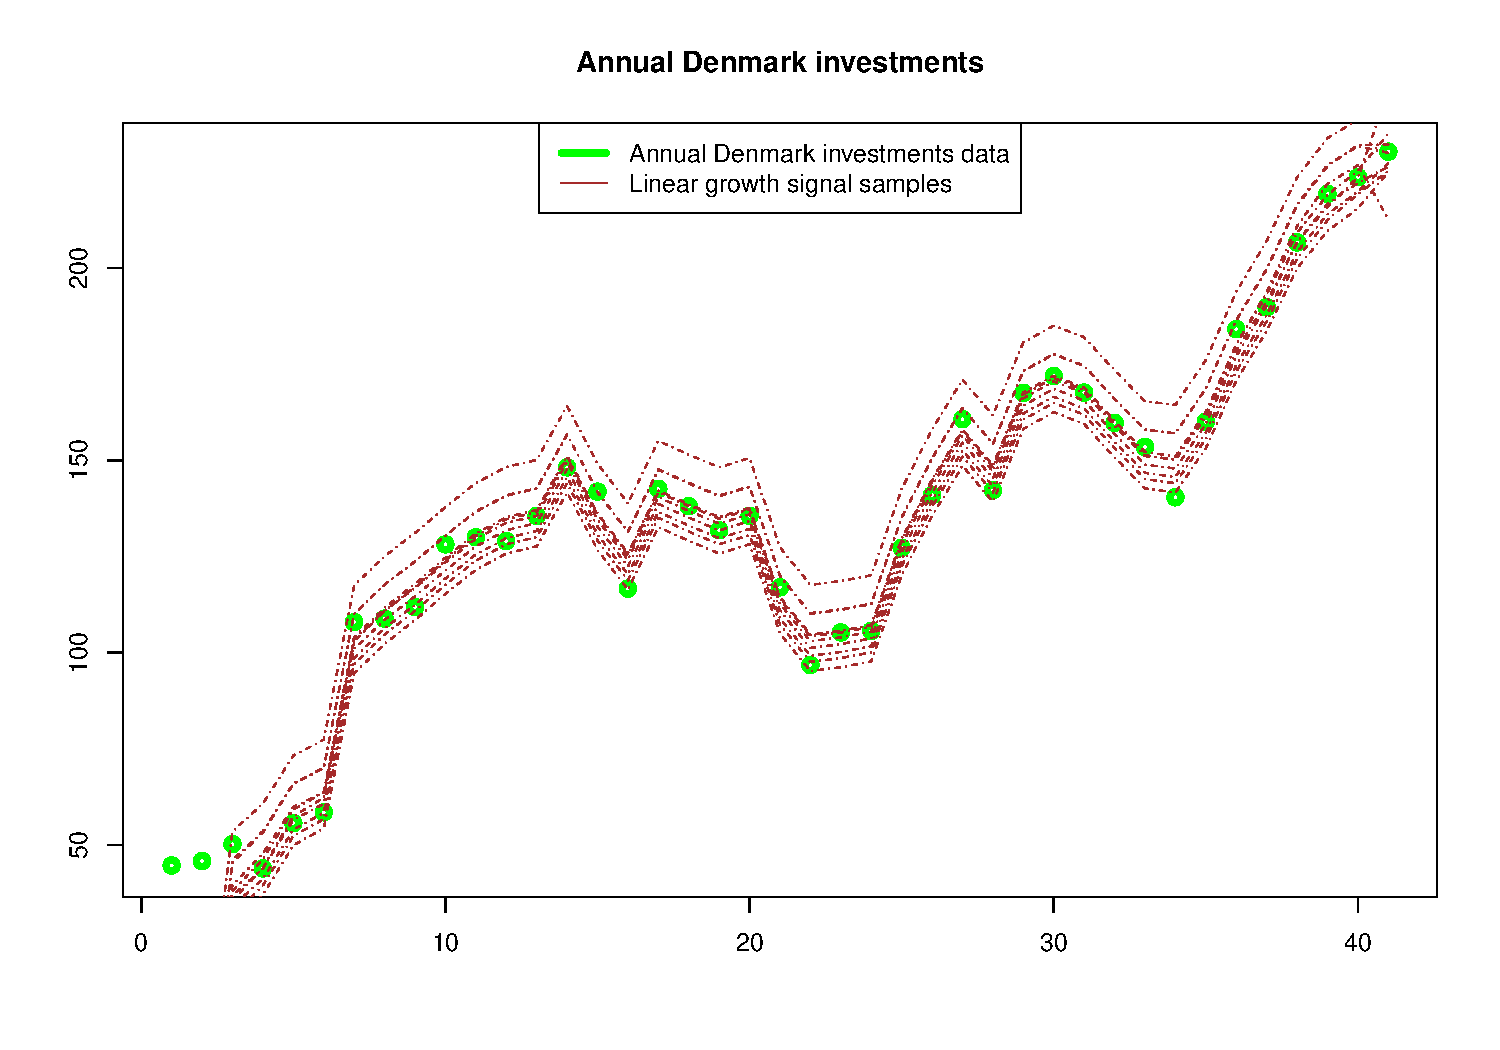
\includegraphics{vignette-027}
\caption{Spain investment data with 10 sampled signal from \GKF}
\label{fig:LGSampleGKF}
\end{figure}

\texttt{dlm} provides the function \texttt{dlm::dlmBSample} to sample from the state
posterior distribution based on the FFBS algorithm. It returns only one sample at a time and
hence needs to be called in a loop if many samples are desired. It only requires the filtered
object (output of \texttt{dlm::dlmFilter}).
\begin{figure}[H]
  \centering
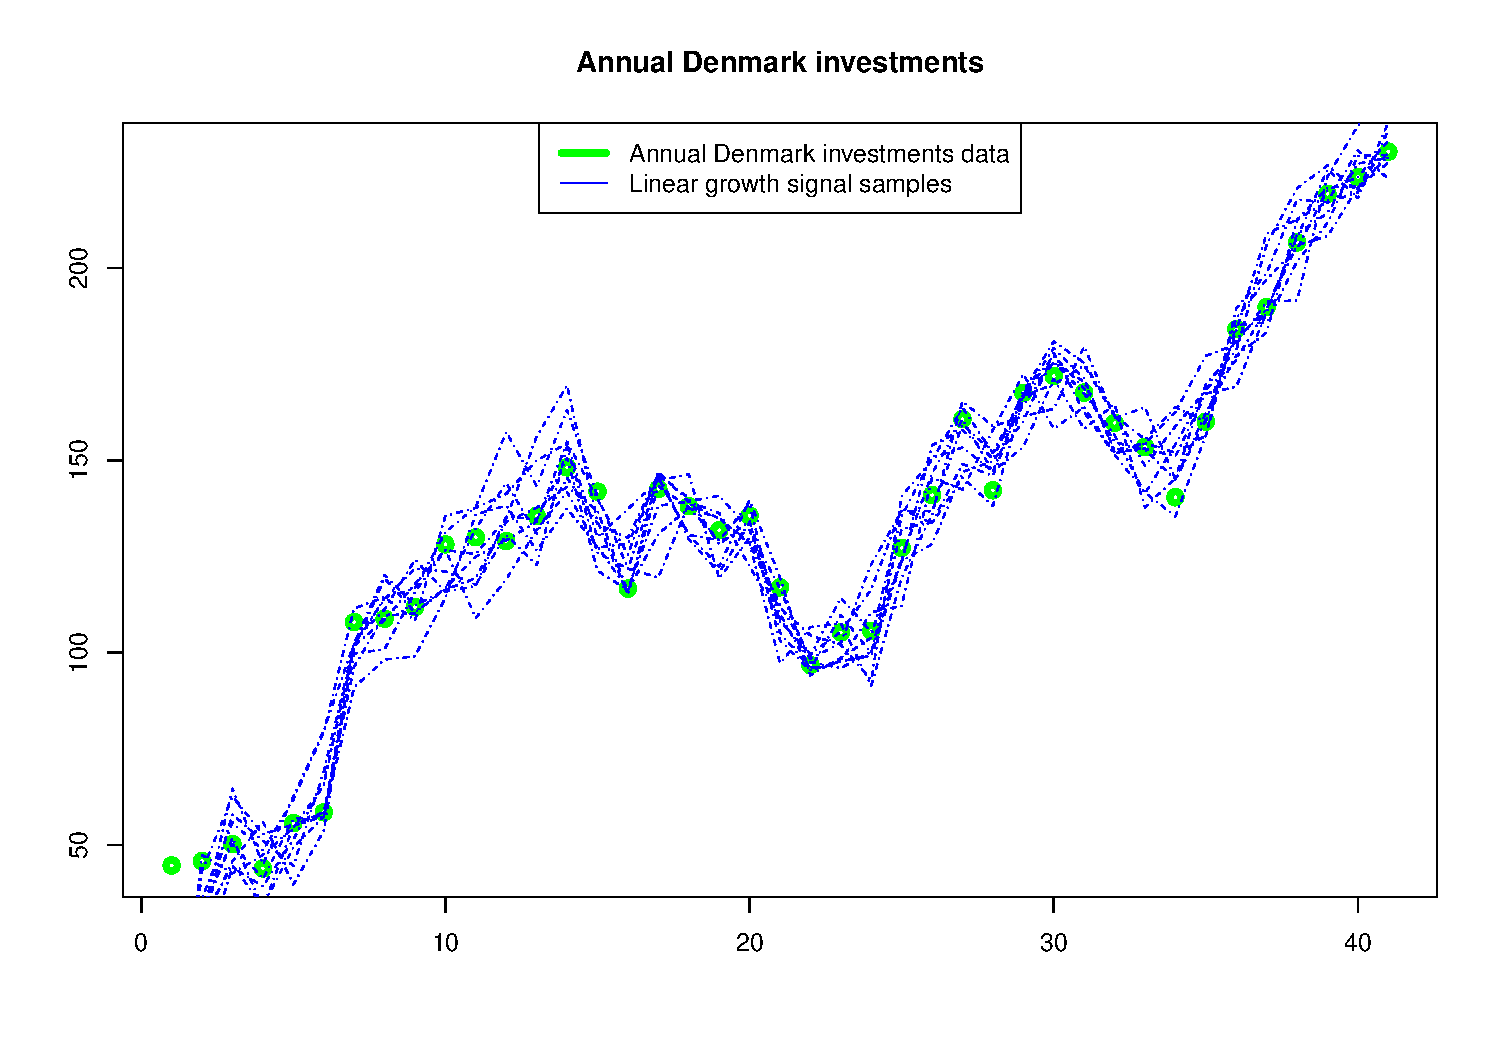
\includegraphics{vignette-028}
\caption{Spain investment data with 10 sampled signal from \texttt{dlm}}
\label{fig:LGSampledlm}
\end{figure}

\section{Additional multivariate example}
\label{sec:additional example}

In this section we discuss the full treatment of an additional multivariate example.

\subsection{A time varying linear Gaussian model: the Dynamic Capital Asset Pricing model}

The capital asset pricing model is used to calculate the required rate of return for any
risky asset (relative to a risk-free asset). A simplified version of the CAPM assumes that
the excess return on a risky asset in any time period is proportional, on average, to the
excess return on a portfolio representing the entire market. The proportionality constants
are known as \textit{betas}.  Considering several assets at once, and allowing the betas to
vary over time, one can set up the following multivariate dynamic regression model
\begin{equation}
  \begin{array}{rccl}
    (r_{a,t} - r_{rf,t}) & = & \beta_t (r_{m,t} - r_{rf,t}) + \epsilon_t  & \epsilon_t \sim \mathcal{N}(0,\Sigma_{\epsilon}) \\
    \beta_{t+1} & = & \beta_t + \eta_t & \eta_t \sim \mathcal{N}(0,\Sigma_{\eta})
  \end{array}
  \label{eq:CAPM}
\end{equation}
where $r_{a,t}$ is the return of the risky asset $a$, $r_{rf,t}$ is the return of the risk
free asset (the reference) and $r_{m,t}$ is the return of the market (an index for example)
at time $t, t=1,\dots,n$. Note that $\Sigma_\epsilon$ and $\Sigma_\eta$ are variance matrices
accounting for correlated observation errors and correlated changes of the betas,
respectively. The data we will use for this example are monthly returns on four stocks
(Mobil, IBM, Weyer, and Citicorp) from January 1978 to December 1987, together with the
30-day Treasury Bill as a proxy for the risk-free asset. The value-weighted average returns
for all the stocks listed at the New York and American Stock Exchanges will be used as a
proxy for the market returns. The data, originally used in \citet{berndt1991practice}, was
collected online \footnote{\url{http://definetti.uark.edu/~gpetris/dlm/}} and are shipped
with package \GKF.

In state space notations, model~\eqref{eq:CAPM} can be summarized in the following system variables:
\begin{equation}
  \begin{array}{rccl}
    y_t =(r_{a,t} - r_{rf,t}) & c_t = 0 & Z_t = (r_{m,t} - r_{rf,t}) I_d & H_t=\Sigma_{\epsilon}   \\
     \alpha_t=\beta_t & d_t=0 & T_t = I_m & Q_t =\Sigma_{\eta}
  \end{array}
  \label{eq:CAPMSS}
\end{equation}
where $m=d=4$ is the number of assets considered. We prepare the data for the analysis first:
\begin{Schunk}
\begin{Sinput}
> data(GKF_data)
> tmp <- GKF.data$CAPMData
> pkDat <- GKF.data$CAPMData
> y <- tmp[, 1:4] - tmp[, "RKFREE"]
> colnames(y) <- colnames(tmp)[1:4]
> market <- tmp[, "MARKET"] - tmp[, "RKFREE"]
> rm("tmp")
> m <- ncol(y)
\end{Sinput}
\end{Schunk}
One can start by estimating the observation and transition variances by maximum
likelihood. We will take advantage of the symmetric property of the matrices by
parameterizing each one in terms of its log Choleski decomposition. Note that the number of
unknown in each matrix is $k=m(m+1)/2=10.$
\begin{Schunk}
\begin{Sinput}
> k <- m*(m+1) * 0.5
> n <- length(market)
> ## Estimate the variances
> yt <- t(y)
> dt = rep(0, m)
> ct = rep(0, m)
> Zt <- sapply(seq_along(market), function(i) market[i] %x% diag(m))
> dim(Zt) <- c(m, m, n)
> Tt = diag(nr = m)
> a0 = rep(0, m)
> P0 = diag(1e7, nr =  m)
> VarLik <- function(theta) {
+     a <- diag(exp(0.5 * theta[1:m]), nr = m)
+     a[upper.tri(a)] <- theta[(m + 1):k]
+     Ht <- crossprod(a)
+     a <- diag(exp(0.5 * theta[1:m + k]), nr = m)
+     a[upper.tri(a)] <- theta[-(1:(k + m))]
+     Qt <- crossprod(a)
+     -FKF(yt = yt, ct = ct, dt = dt, Zt = Zt, Tt = Tt,
+          Ht = Ht, Qt = Qt, a0 = a0, P0 = P0)$logLik
+ }
> fit <- optim(par = rep(0, 2 * k),fn = VarLik, method = "BFGS",
+              control = list(maxit = 500))
> theta <- fit$par
> a <- diag(exp(0.5 * theta[1:m]), nr = m)
> a[upper.tri(a)] <- theta[(m+1):k]
> Ht <- crossprod(a)
> a <- diag(exp(0.5 * theta[1:m + k]), nr = m)
> a[upper.tri(a)] <- theta[-(1:(k + m))]
> Qt <- crossprod(a)
\end{Sinput}
\end{Schunk}
The next step is to compute the betas from the smoothed signal in the usual way by a call to
the \texttt{GaussianSignalSmoothing} function
\begin{Schunk}
\begin{Sinput}
> smoothCAPM <- GaussianSignalSmoothing(yt = yt, ct = ct, dt = dt, Zt = Zt, Tt = Tt,
+                                       Ht = Ht, Qt = Qt, a0 = a0, P0 = P0)
> thetas <- t(smoothCAPM$theta)
> betas <- matrix(0, n, m)
> for (i in 1:length(market))  betas[i, ] <- t(solve(Zt[, , i])%*%thetas[i, ])
> betas <- ts(betas, start = start(market), freq = frequency(market))
\end{Sinput}
\end{Schunk}

Except for the Mobil stock, Figure~\ref{fig:betas} (page~\pageref{fig:betas}) shows that all the other betas changes considerably over time which justifies the dynamic assumption.
\begin{figure}[htbp]
  \centering
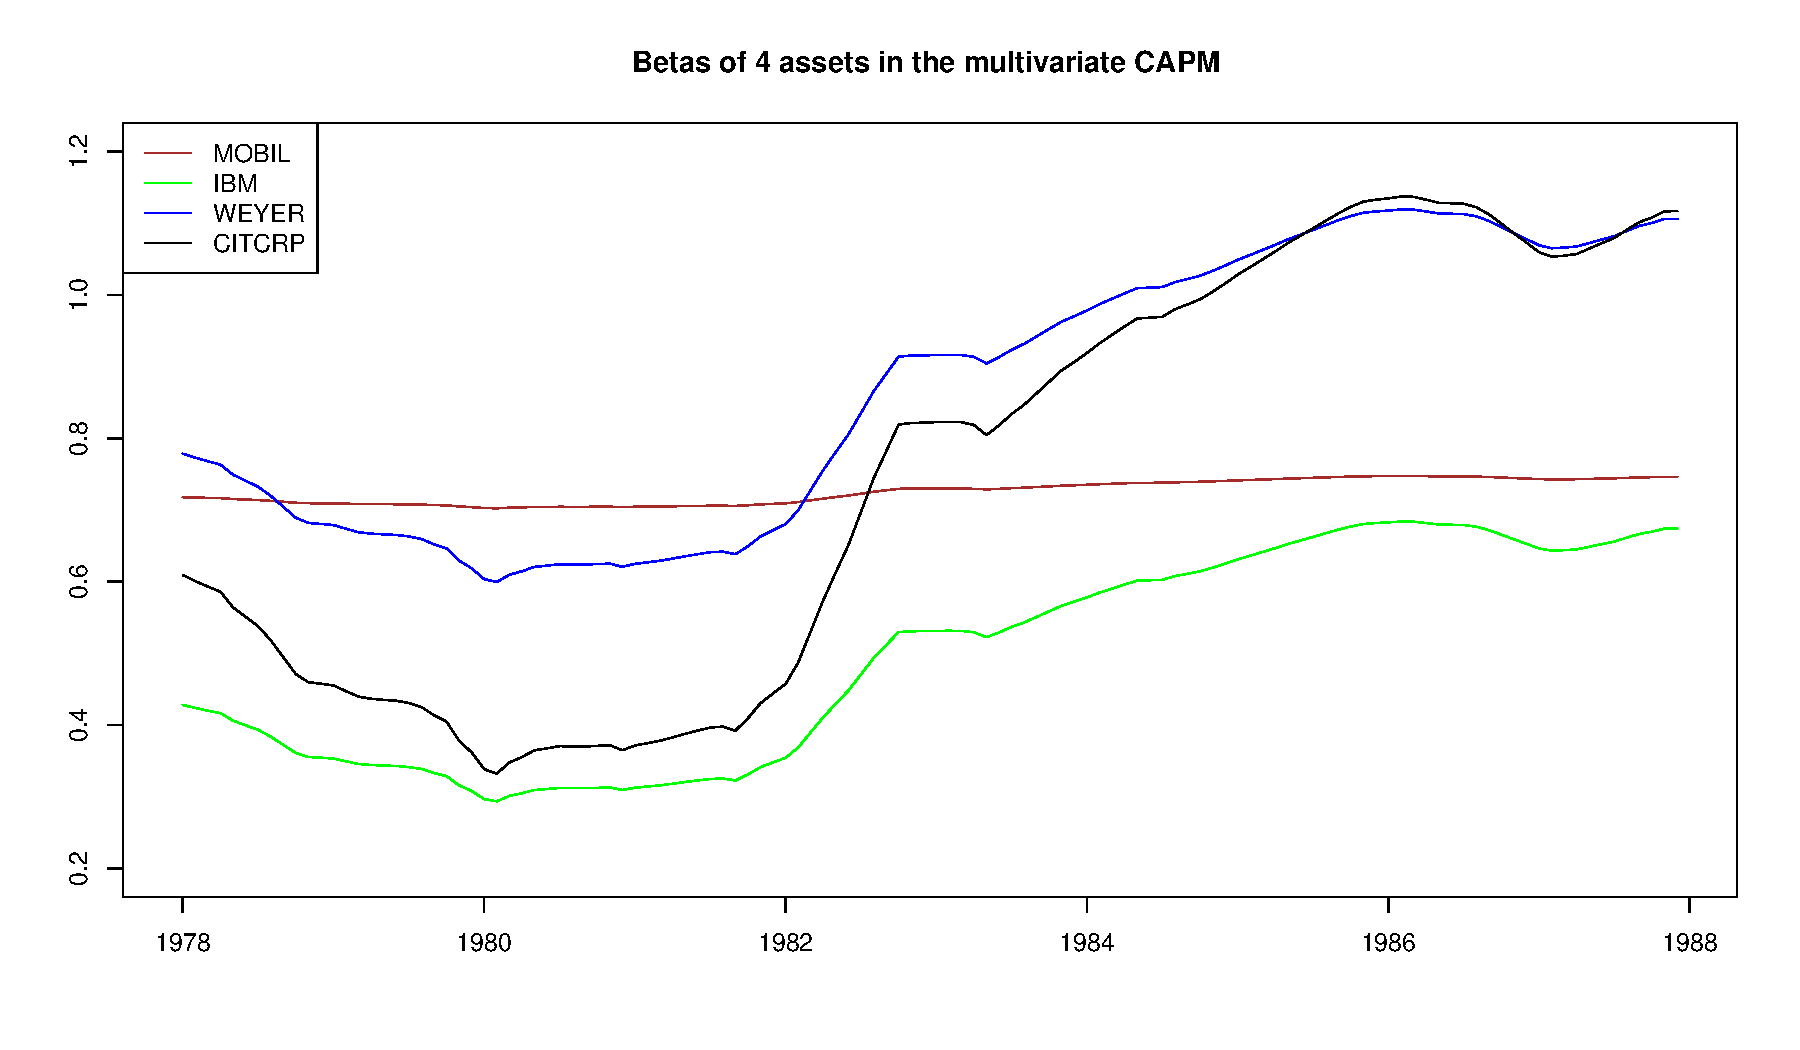
\includegraphics{vignette-032}

\caption{Multivariate dynamic CAPM : betas visualization}
\label{fig:betas}
\end{figure}

If a sample from the posterior distribution of the betas is desired, one needs to call
\texttt{GaussianthetaSampling} with the usual inputs. Figure~\ref{fig:sampleIBM}
(page~\pageref{fig:sampleIBM}) illustrates this task for the IBM stock:
\begin{figure}[htbp]
  \centering
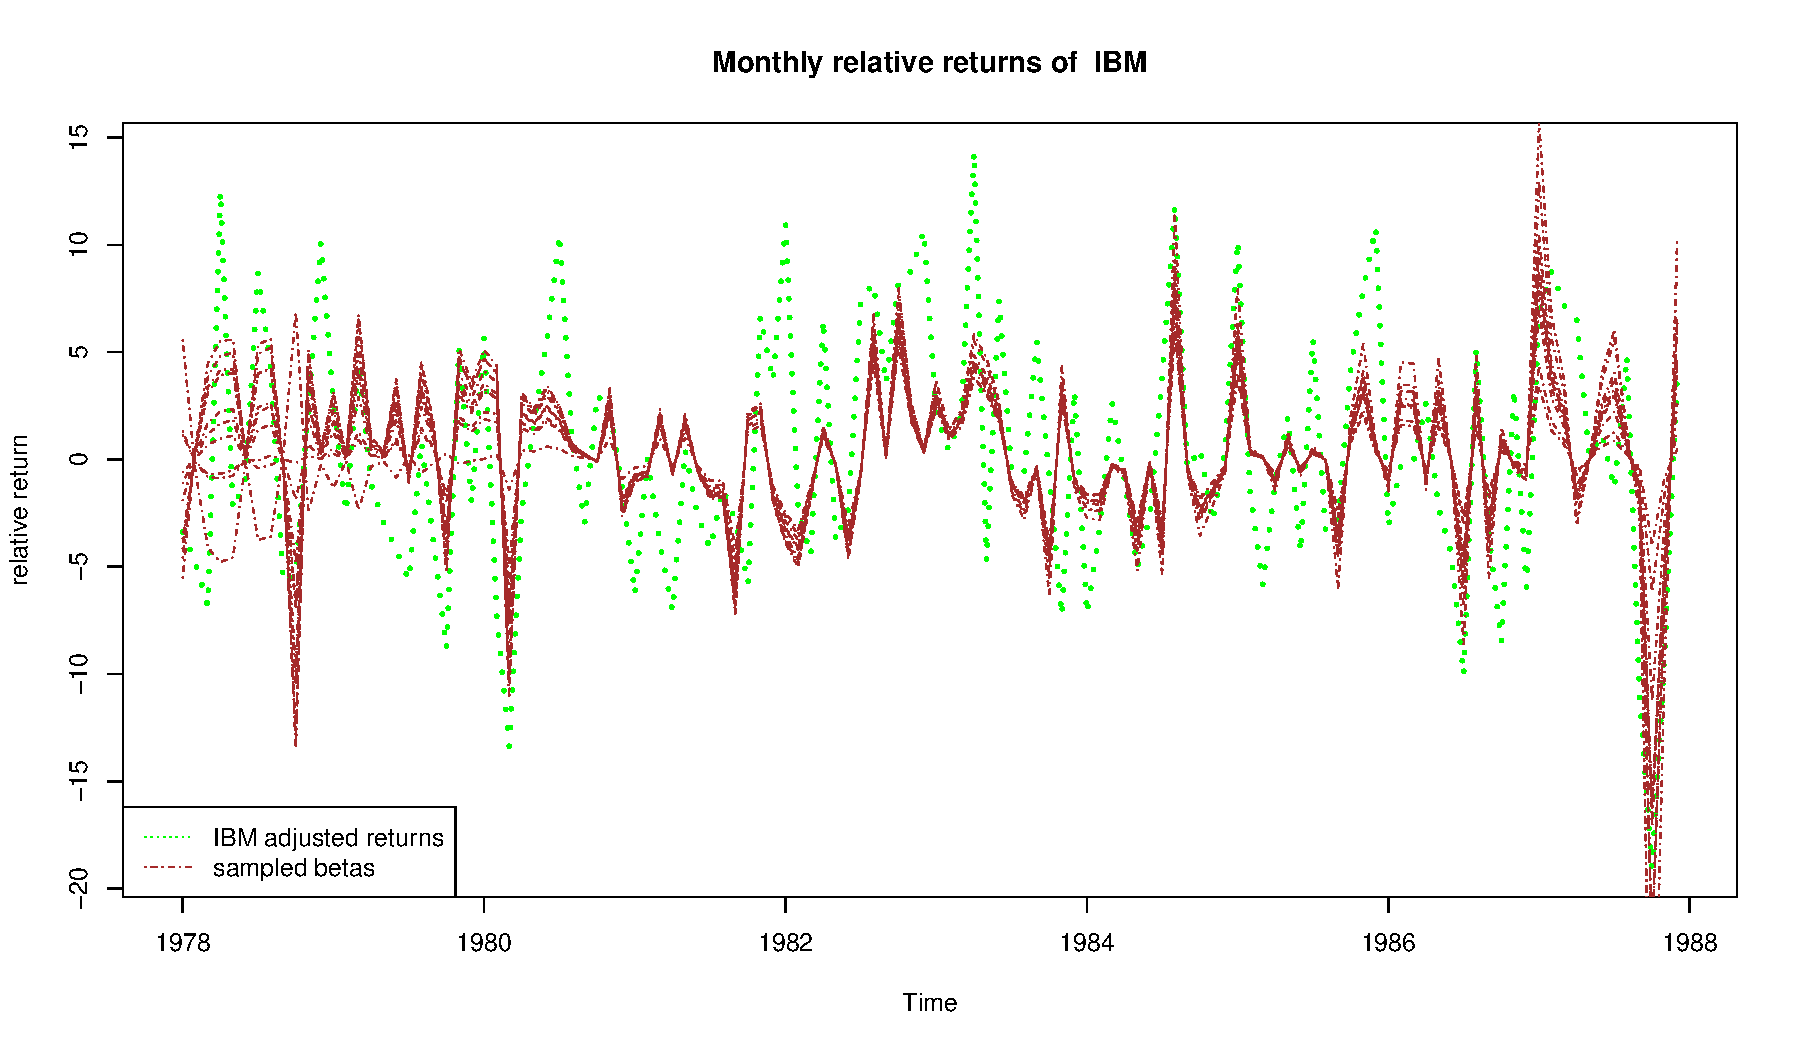
\includegraphics{vignette-033}
\caption{10 samples from the posterior signal distribution of IBM returns together with the real data.}
\label{fig:sampleIBM}
\end{figure}

\section{A nonLinear non-Gaussian example: the Poisson scoring model}
\label{sec:nLnGaussian}

In the nonlinear non-Gaussian case, the simplfying Gaussian assumption drops and hence
computation is slightly more complicated. The model considered here is the transition
Equation~\eqref{eq:Transition} together with the observation
Equation~\eqref{eq:measurementH}.

\subsection{Computing the posterior mode}

We first note that the filtering and smoothing operations described before are equivalent to
the computation of the posterior mode of $p(\theta_t|y_1,\dots,y_t)$ and
$p(\theta_t|y_1,\dots,y_n)$ respectively (together with the associated Hessian matrix). For
non-Gaussian models, these computations are usually not doable in analytical form but can be
obtained by maximization of $p(\theta_*|y)$ using for example the Newton-Raphson
algorithm. This approach was suggested by \citet{jungbacker2007monte} and is the one
implemented in \GKF.

For a given guess $g$ of the optimum $\hat{\theta}$, the Newton-Raphson method proposes the
updated guess $g^+$ defined by
\begin{equation*}
  g^+ = g -\{ \ddot{p}(\theta|y)|_{\theta=g} \}^{-1} \dot{p}(\theta|y)|_{\theta=g}
  ,
\end{equation*}
where $ \dot{p} (.|.) = \frac{\partial \log p (.|.)}{ \partial \theta}$ and $ \ddot{p} (.|.) = \frac{\partial^2 \log p (.|.)}{ \partial \theta \partial \theta^{\prime}}$.
It can be shown that the updating step can be written as
\begin{align}
    g^+ &= g - \{\ddot{p}(y|\theta)|_{\theta=g} - \Psi^{-1}  \}^{-1} \{
          \dot{p}(y|\theta)_{\theta=g} - \Psi^{-1} (g- \mu) \} \nonumber \\
        &= (\Psi^{-1} + A^{-1})^{-1} (A^{-1} x + \Psi^{-1} \mu)
  ,
  \label{eq:NewtonStep}
\end{align}
where $ A = - \{\ddot{p}(y|\theta)|_{\theta=g} \}^{-1} $ and $x=g + A \dot{p}(y|\theta)_{\theta=g}$, $\Psi$ and $\mu$ defined in \eqref{eq:SignalVec}.

If we can assure that $\ddot{p}(y|\theta)|_{\theta=g} $ is negative definite for all values
of $\theta$, the Kalman filter and smoother recursions can be used to compute $g^+$ by taking
model \eqref{eq:Transition}-\eqref{eq:measurement} with $y=x$ and $H=A$. Note that the
Hessian is simply given by
$ G= \{\ddot{p}(\theta|y)|_{\theta=\hat{\theta}} \}^{-1} = -\Psi^{-1} - A^{-1}$. However, if
this assumption cannot be made, \citet[Theorem~1]{jungbacker2007monte} state that a Kalman
filter similar approach could be used to compute $g^+$. The suggested algorithm is summarized
below:
\begin{itemize}
\item First, compute the Kalman filter forward recursions with $y_t=x_t $ and $H_t=A_t$
  (where $x$ and $A$ are defined by Equation~\eqref{eq:NewtonStep})
  \begin{equation}
  \begin{array}{rcl}
    v_t = x_t - c_t - Z_t \alpha_t, &  F_t = A_t + Z_t P_t Z_t^{\prime}, & \\
     & K_t=T_t P_t Z_t^{\prime} F_t^{-1}, & t=1,\dots,n, \\
     \alpha_{t+1}=d_t + T_t \alpha_t + K_t v_t, & P_{t+1}=T_t P_t T_t^{\prime}-K_t F_t K_t^{\prime}+ Q_t,
  \end{array}
  \label{eq:KFForward}
\end{equation}

\item Then, carry out the following backward recursion using quantities previously computed.
   \begin{equation}
  \begin{array}{rcl}
    e_t = F_t^{-1} v_t - K_t^{\prime} s_t, &  & s_{t-1} = Z_t^{\prime} e_t + T_t^{\prime}s_t, \\
     &  g_t^+ = x_t -A_t e_t  &
  \end{array}
  \label{eq:KFBackward}
\end{equation}
for $t=n,\dots,1$ with initialization $s_n=0$.
\end{itemize}

Function \texttt{NRUpdatingStep} implements this procedure and is called iteratively until
convergence in function \texttt{ PosteriorSignalMode} to obtain the posterior mode
$\hat{\theta}$.

\subsection{Sampling from the proposal density}
\label{sec:SamplingNonLin}

In the nonlinear non-Gaussian case, it is usually not feasible to sample from
$p(\theta|y,\psi)$. Hence one needs to find a density $f(\theta |y,\psi)$ that is similar to
$p(\theta|y,\psi)$ and from which samples can be obtained efficiently. This density is known
as the proposal density. \GKF implements a Gaussian proposal density with the same mode as
the target and with the same curvature around the mode that is
\begin{equation}
  \begin{array}{rcl}
    f(\theta|y,\psi)=\mathcal{N} (\hat{\theta},V), & V= -G^{-1}, & G = \{\ddot{p}(\theta|y)|_{\theta=\hat{\theta}} \}^{-1} = -\Psi^{-1} - A^{-1}
  \end{array}
  \label{eq:NewtonStepSample}
\end{equation}
where $A$ is defined as before and evaluated at $\theta=\hat{\theta}$.

Again, if we can assure that $A$ is positive definite, the linear Gaussian sampling method of
\citet{durbin2002simple} (\GKF function \texttt{GaussianthetaSampling}) can be called with
$y=\hat{\theta} + A \dot{p}(y|\theta)|_{\theta=\hat{\theta}}$ and $H=A$. If this assumption
cannot be made, one can use \citet[Theorem~2]{jungbacker2007monte} which only requires
$\ddot{p}(\theta | y)$ to be invertible. If we define $A$ as in \eqref{eq:NewtonStepSample}
and $x=\hat{\theta} + A \dot{p}(y|\theta)|_{\theta=\hat{\theta}}$, a sample $\theta^i$ from
the proposal density $f(\theta|y,\psi)$ defined in \eqref{eq:NewtonStepSample} is generated
by first computing \eqref{eq:KFForward} at the $x$ points along with the following recursions
% \begin{equation}
%   \begin{array}{rl}
%     C_t=A_t^{-1} - F_t^{-1} -K_t^{\prime}N_t K_t,& R_t= C_t^{-1}(A_t^{-1} Z_t - K_t^{\prime}N_t T_t), \\
%     \omega_t \sim \mathcal{N}(0,C_t) ,& u_t = A_t=(\omega_t + F_t^{-1} v_t - K_t^{\prime}r_t), \\
%     r_{t-1}= Z_t^{\prime} A_t^{-1}u_t - R_t^{\prime} \omega_t + T_t^{\prime}r_t, &
%     R_{t-1}= R_t^{\prime}C_t R_t - Z_t^{\prime}A_t^{-1}Z_t + T_t^{\prime}N_tT_t ,
%   \end{array}
%   \label{eq:SimSmootherAlgo}
% \end{equation}
\begin{equation}\label{eq:SimSmootherAlgo}
\begin{aligned}
       C_t &= A_t^{-1} - F_t^{-1} -K_t^{\prime}N_t K_t
    ,& R_t &= C_t^{-1}(A_t^{-1} Z_t - K_t^{\prime}N_t T_t), \\
      \omega_t &\sim \mathcal{N}(0,C_t)
    ,& u_t &= A_t=(\omega_t + F_t^{-1} v_t - K_t^{\prime}r_t), \\
       r_{t-1} &= Z_t^{\prime} A_t^{-1}u_t - R_t^{\prime} \omega_t + T_t^{\prime}r_t
    ,& R_{t-1} &= R_t^{\prime}C_t R_t - Z_t^{\prime}A_t^{-1}Z_t + T_t^{\prime}N_tT_t
    ,
\end{aligned}
\end{equation}
for $t=n,\dots,1$ with usual initialization $r_n=0$ and $N_n=0$. The simulation $\theta^i$
from $f(\theta|y,\psi)$ is obtained by
$ \hat{\theta} + (u_1^\prime,\dots,u_n^\prime)^\prime$.  This method is implemented in \GKF
(function \texttt{PosteriorSignalSampling}) and allows users to generate more than one
sample. It is recommended to set the seed before sampling especially if the samples will be
used in importance sampling (or any similar simulation based estimation method).

Assume a sample $\theta^i$ is obtained from $f(\theta|y,\psi) = \mathcal{N}(\hat{\theta},V)$
using \eqref{eq:SimSmootherAlgo}. The log-density $\log(f(\theta^i|y,\psi))$ is given by
\begin{equation}
   \log(f(\theta^i|y,\psi)) = -\frac{dn}{2} \log{2 \pi} - \displaystyle \sum_{t=1}^n \log{|\text{det}A_t|} - \displaystyle \sum_{t=1}^n \log{(\text{det}B_t)} - \frac{1}{2} \displaystyle \sum_{t=1}^n b_t^{i \prime} b_t^{i},
  \label{eq:logLikSimSampl}
\end{equation}
where $b_t^{i}$ and $B_t$ implicitely defined as $ \omega _t^i = B_t b_t^i $ and
$C_t=B_tB_t^\prime$, respectively. \citet{jungbacker2007monte} proved that the matrix $C_t$
is definite semi-positive however, numerical instabilities may appear and abort the
computation if $C_t$ is not carefully checked before using it, see Section~\ref{App:Nearest}
for more details.

\subsection{Likelihood evaluation}
\label{sec:ImportanceSamplingLik}

We noted previously that some system vectors and matrices can depend on a vector of parameter
$\psi$. Following \citet{durbin2012time}, we opt for the method of maximum likelihood to
estimate the parameters collected in $\psi $ which produces optimal properties in large
samples.

The likelihood function for the vector of observation $y$ is based on the observation density
and the time independence assumption \eqref{eq:measurementH} and is given by
\begin{equation}
   L(\psi)=p(y|\psi)= \int p(y,\theta|\psi)d\theta = \int p(y|\theta,\psi) p(\theta|\psi)dz
  \label{eq:logLikPsi}
\end{equation}
which needs to be evaluated at different values of the parameter vector $\psi$ in reasonable
computing times as it will be called several times by the optimization routine. An analytical
solution to evaluate the previous integral is not available and hence numerical evaluation
will be considered. It is well established that numerical integration in multi-dimensional
space becomes quickly infeasible when the dimension increases. Consequently, we will adopt
simulation based techniques. Given that we know how to draw samples from $p(\theta|\psi) $
and have usually explicit expression for $p(y|\theta,\psi)$, one may think that the problem
can be solved by 'direct' Monte Carlo estimate as follows:
\begin{itemize}
\item draw $M$ independent samples $\theta^{(k)}$ from $p(\theta|\psi)$

\item get the estimate $\hat{L}(\psi)$ by avereging $p(y|\theta^{(k)},\psi)$, i.e,
  $\hat{L}(\psi) = \displaystyle \sum_{k=1}^M \frac{1}{M} p(y|\theta^{(k)},\psi)$
\end{itemize}
However, as highlighted in figure~\ref{fig:DiffSample}, sampling unconditionnally on the data
is not efficient and hence leads to poor estimates. A more effective approach is based on
impotance sampling as advocated by \citet[see][chap. 11]{durbin2012time}. Starting from
\eqref{eq:logLikPsi}, we can modify the likelihood
% \begin{equation}
%   \begin{array}{rccl}
%    L(\psi) & = & p(y|\psi) = & \int p(y,\theta|\psi)d\theta \\
%            &   &            & \\
%            &   &           = & \int p(y|\theta,\psi) p(\theta|\psi)dz \\
%            &   &            & \\
%            &   &           = & \int \frac{p(y|\theta,\psi) p(\theta|\psi)}{p(\theta|y,\psi)} p(\theta|y,\psi) dz \\
%            &   &            & \\
%            &   &           = & \E \Big ( \frac{p(y|\theta,\psi) p(\theta|\psi)}{p(\theta|y,\psi)} \Big )_p
%   \label{eq:logLikPsiImpotance}
%   \end{array}
% \end{equation}
%
\begin{comment}
  G: (1) Tarak, you may wish to use more environment align or aligned. I have changed it at a
  couple of places as an example. Here I used ``aligned'' to mimic your layout but it may be
  better to use ``align'' and number only the last row. To leave more space between lines,
  use the option argumnent of \verb+\\+, as in the last line below.

  (2) It is more usual to write $E_{p}(...)$ rather than $E(...)_{p}$
\end{comment}
\begin{equation}\label{eq:logLikPsiImpotance}
\begin{aligned}
  L(\psi)
      = p(y|\psi)
     &= \int p(y,\theta|\psi)d\theta
  \\ &= \int p(y|\theta,\psi) p(\theta|\psi)dz
  \\ &= \int \frac{p(y|\theta,\psi) p(\theta|\psi)}{p(\theta|y,\psi)} p(\theta|y,\psi) dz
  \\[5pt] &= \E \Big ( \frac{p(y|\theta,\psi) p(\theta|\psi)}{p(\theta|y,\psi)} \Big )_p
\end{aligned}
\end{equation}
where $\E ()_p$ denotes expectation with respect to density $p(\theta|y,\psi)$. This
expectation can be evaluated in the usual way by sampling from $p(\theta|y,\psi)$ and
averaging the importance weights
$q=\frac{p(y|\theta,\psi) p(\theta|\psi)}{p(\theta|y,\psi)}$. To summarize, the importance
sampling estimate is given by
\begin{equation}
  \begin{array}{rcl}
   \hat{L}(\psi) = \frac{1}{M} \displaystyle \sum_{i=1}^M q_i, & q_i=\frac{p(y|\theta^i,\psi) p(\theta^i|\psi)}{p(\theta^i|y,\psi)}, & \theta^i \sim p(\theta|y,\psi),
   \end{array}
   \label{eq:ImportanceSamplEq}
\end{equation}
where $q_i$ is referred to as an important weight, which can be computed using
\eqref{eq:measurementH}, \eqref{eq:logLikSimSampl} and ideas discussed in Appendix
\ref{App:logLikCompute}. The samples $\theta^i$ are obtained from the sampling smoother
algorithm described in \ref{sec:SamplingNonLin}. For purpose of likelihood maximisation with
respect to $\psi$, it is preferred to work with the log-likelihood function. However, taking
the logarithm in~\eqref{eq:ImportanceSamplEq} introduces bias that can be accounted for as
explained in Appendix~\ref{App:logLikBias}.

\subsection{ A nonlinear non-Gaussian example}

\subsubsection{The model}

The example selected is a simple model to forecast the number of goals scored (build a
probabilty table for all possible outcomes) by a football team based on its past
performance. We assume that the number of goals scored by a team can be modelled by a Poisson
process where the (log)intensity follows a Markovian process
\begin{equation}
  \begin{array}{rcl}
    \Prob(y_t=x |\lambda_t) & = & \text{Poiss} (\lambda_t) \\
    \lambda_t & = & \exp(\alpha_t) \\
    \alpha_{t+1} & = &  \phi_{\alpha} \alpha_{t} + \eta_{\alpha,t}
  \end{array}
  \label{eq:PoissModel}
\end{equation}
Model~\eqref{eq:PoissModel} considers only one team scoring process. If more than one team
($k$ teams) is of interest, the associated multivariate model can be obtained as follows. Let
$y_t = (y_{1,t},\dots, y_{k,t}) $ be the number of goals scored by the $k$ teams at time $t$
and define the intensity $\lambda_t$ and state (equal to the signal in this case) vectors
similarly. Assuming independence between goals \footnote{We are fully aware that this
  assumption is not verified in reality. In fact, if team A plays team B, the goals scored by
  team A is highly influenced by the goals scored by team B. However, the aim of this example
  is illustrative and hence we assumed independence to keep things simple.} scored by each
team at time $t$, one gets
\begin{equation}
  \begin{array}{rcl}
    \Prob(y_t|\alpha_t) & = & \displaystyle \prod_{i=1}^k \text{Poiss} (\lambda_{t,i}) \\
    \lambda_{t,i} & = & \exp(\alpha_{t,i}), \ i=1,\dots,k \\
    \alpha_{t+1} & = &  \Phi_{\alpha} \alpha_{t} + \eta_{\alpha}
  \end{array}
  \label{eq:PoissModel1}
\end{equation}
where $\Phi_{\alpha} =\text{diag}(\phi_\alpha)$ and
$\eta_{\alpha} \sim \mathcal(0,Q), \ Q=\text{diag}(\sigma^2) $.  Assuming independence
between the $n$ time observations and defining $y=(y_1 ^\prime, \dots, y_n^\prime)^\prime$
and similarly $\alpha= (\alpha_1 ^\prime, \dots, \alpha_n^\prime)^\prime$, we get :
$ \Prob(y|\alpha;\psi)= \displaystyle \prod_{t=1}^n \Prob(y_t|\alpha_t;\psi)$ where $\psi$ is
the vector of parameters defined as $\psi=(\phi,\sigma^2)$ which can be easily computed in \R
by
\begin{Schunk}
\begin{Sinput}
> dP <- function(theta,y){
+     lambda <- exp(theta)
+     sum(dpois(as.numeric(y), as.numeric(lambda), T), na.rm = TRUE)
+ }
\end{Sinput}
\end{Schunk}
Note that the function should accept \texttt{NA} values and only return \texttt{numeric}
which was done in \texttt{dP} by setting \texttt{na.rm=TRUE} in \texttt{dpois}.

\subsubsection{The data}

The data collects the goals scored in games between 10 selected English Premier League
football teams \footnote{Arsenal, Aston Villa, Chelsea, Everton, Fulham, Liverpool, Man City,
  Man United, Tottenham, Wigan.} from season 2005-2006 to season 2012-2013 which gave us 180
($10 \times 9 \times 2)$ observation per season. The data was divided in 2 sets. A short one
with only 2 seasons (2011-2012 / 2012-2013) called \texttt{shortGoals} and the longer one
with the entire dataset called \texttt{longGoals} \footnote{the data is available at
  \url{http://www.football-data.co.uk/}}.

\subsubsection{Study a nonlinear non-Gaussian model with \GKF}

As discussed earlier, in order to fit a nonlinear non-Gaussian model one needs to provide the
first and second derivatives of the conditional log-density $p(y|\theta)=p(y|\alpha)$. Those
derivatives are given in this example by:
\begin{equation*}
  \dot{p}(y_t|\theta_t)
  = y_t -\exp(\theta_t) \ , \ \ddot{p}(y_t|\theta_t)=\text{diag}( -\exp(\theta_t))
\end{equation*}
and can be defined in \R as follows:
\begin{Schunk}
\begin{Sinput}
> jac_ <-  function(theta, y, Pars = list()) {
+     res <- y - exp(theta)
+     res[is.na(res)] = 0
+     res
+ }
> hess_ = function(theta, y, Pars = list()) diag(-exp(theta))
\end{Sinput}
\end{Schunk}
Note the extra parameter \texttt{Pars} in these functions. \texttt{Pars} is used to pass
extra inputs, when needed, to compute the derivatives. Morever, both routines need to handle
missing values in $y$. We recommand to set the derivative component related to a missing
value $y_{t,k}$ to 0. In the previous example, only the first derivative deals with missing
values because the hessian expression is independent of $y$.

The model is then built up, the data-set selected and the parameters $\phi =0.9975$ and
$\sigma^2=0.000205$ are specified.
\begin{Schunk}
\begin{Sinput}
> data(GKF_data)
> yt.long <- GKF.data$longGoals
> yt.short <- GKF.data$shortGoals
> d <- nrow(yt)
> n <- ncol(yt)
> m <- d
> phi <- 0.9975
> sig2 <- 0.000205
> P0 <- diag(sig2, m, m)
> a0 <- numeric(m)
> Zt <- diag(1, d, m)
> dt <- numeric(m)
> ct <- numeric(d)
> Tt <- diag(phi, m, m)
> Qt <- diag(sig2, m, m)
\end{Sinput}
\end{Schunk}

A more interesting example considers the vector of parameters $\psi$ unknown and estimates it by maximum likelihood based on importance sampling as described in Section~\ref{sec:ImportanceSamplingLik}. The requirements for this method are the following
\begin{enumerate}
\item Provide a routine to compute the log-likelihood. The first argument of this function
  should be the parameter \texttt{psi}. Other inputs are the seed used to generate the
  importance sample, the observation matrix and the number of sample used. Note that the seed
  is required to be the same for the generation of the \texttt{M} simulated paths of $\theta$
  in order to obtain a smooth multi-dimensional likelihood surface in $\psi$ for its
  maximization \citep{jungbacker2007monte}. Although small, the bias correction needs to be included if the logarithm of the importance weights is used directly in the estimator, see Appendix~\ref{App:logLikBias}.
\begin{Schunk}
\begin{Sinput}
> computeLogLik <- function(psi, seed=345, yt=yt.long, M=50){
+     set.seed(seed)
+     phi <- psi[1]
+     sig2 <- psi[2]
+ 
+     ## dim
+     d <- nrow(yt)
+     n <- ncol(yt)
+     m <- d
+ 
+     ## dlm objects
+     P0 <- diag(sig2, m, m)
+     a0 <- numeric(m)
+     Zt <- diag(1, d, m)
+     dt <- numeric(m)
+     ct <- numeric(d)
+     Tt <- diag(phi, m, m)
+     Qt <- diag(sig2, m, m)
+ 
+     thetaSample <- PosteriorSignalSampling(a0, P0, dt, ct, Tt, Zt, Qt, yt,
+                                            SpecificPars = list(jac = jac_, hess = hess_),
+                                            M = M, type = "NLnonGaussian")
+     loglikV <- numeric(M)
+     for (i in 1:M){
+         thSample <- thetaSample$theta[, , i]
+         loglikV[i] <- dP(thSample, yt) + thetaSample$UncondthetaLogLik[i] -
+                                          thetaSample$CondthetaLogLik[i]
+     }
+     bias.corr <- log(1 + var(loglikV) / (2*M))
+     return(- mean(loglikV) - bias.corr )
+ }
\end{Sinput}
\end{Schunk}

\item Choose an optimization routine together with an initial guess for $\psi$. Following
  standard procedure, we minimize the inverse log-liklihood instead of maximizing the
  (log-)likelihood. We have tried several optimization algorithms (using the \texttt{optimx}
  wrapper \citep[see ]{optimx2014}). We found that the \R box-constrained optimization using
  PORT routines \texttt{mlminb} works best (smallest objective value, minimum number of
  iterations and shortest execution time).
\begin{Schunk}
\begin{Sinput}
> phi <- 0.5
> sig2 <- 1
> Par <- nlminb(start = c(phi, sig2),  objective = computeLogLik,
+               lower = c(1e-3, 1e-3), upper = c(1, 4))
> MLParams <- Par$par
> phi <- MLParams[1]
> sig2 <- MLParams[2]
\end{Sinput}
\end{Schunk}
\end{enumerate}
To illustrate the result, we can use the estimated parameters to construct the posterior
signal mode (best estimate of the signal), convert it to scoring intensity (just apply the
exponential) and then plot the scoring intensity for a given team (by setting the
\texttt{team_index} to a number between 1 and 10) together with the observed scored
goals. Recall that the scoring intensity in a Poisson model coincides with its expected value
(the mean).
\begin{Schunk}
\begin{Sinput}
> thetaHat <- PosteriorSignalMode(a0, P0, dt, ct, Tt, Zt, Qt, yt,
+                                 jac_, hess_, list(), 0)$theta_hat
> lambdaHat <- exp(thetaHat)
> teams <- rownames(lambdaHat)
\end{Sinput}
\end{Schunk}

\begin{figure}[htbp]
  \centering
 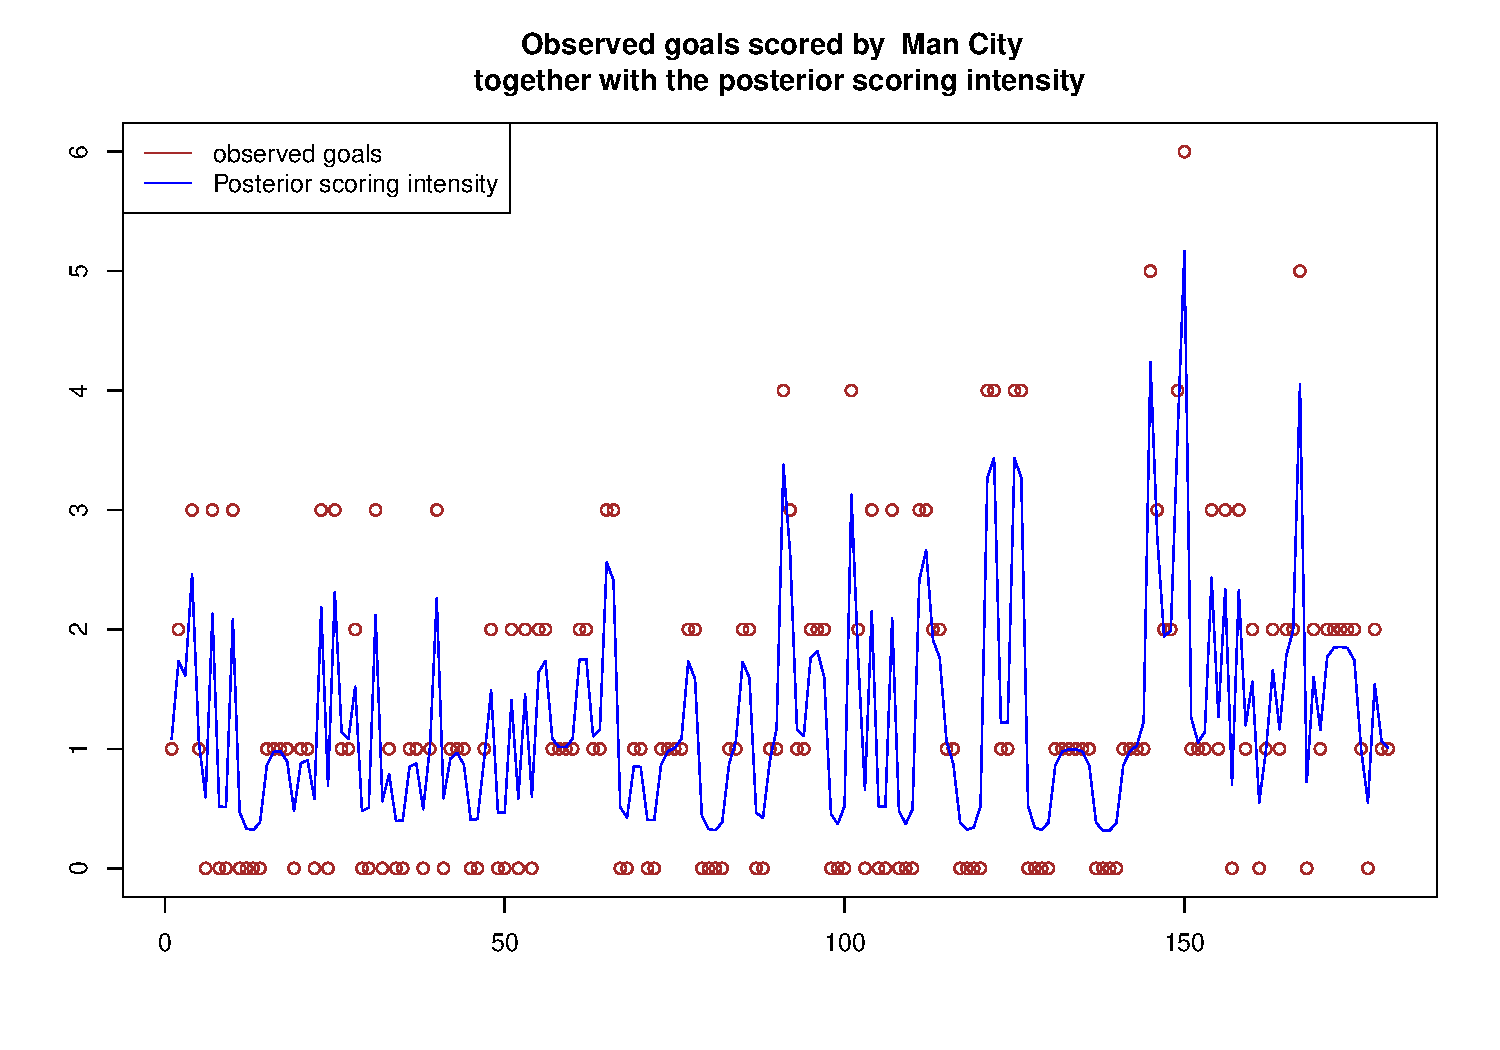
\includegraphics{intensity.pdf}
\caption{Manchester City observed scored goals plotted against its AR-Poisson scoring intensity}
\label{fig:SCIntensityVSObserved}
\end{figure}

Figure ~\ref{fig:SCIntensityVSObserved} shows that the scored goals highly fluctuates over
time whcih makes a constant scoring intensity unrealistic. Althought simple, the dynamic
AR-Poisson model renders better the evolution of the scoring process and can be considered as
a good improvement to the static Poisson counting process. Readers interested in a more
elaborated model for forecasting football match results are referred to
\citet{koopman2013dynamic}.

\section{Conclusion}
\label{sec:CL}

In this paper we introduce the different functionalities available in package \GKF. To our
knowledge, \GKF is the first \R package to offer facilities to fit non linear non-Gaussian
models when the observations are not assumed to come from a log-concave density. Most of the
computation in \GKF are done in \texttt{C++} which makes it fast enough to be able to fit
high-dimensional state space models to large datasets. We showed in this paper different
examples and how \GKF can be used to fit them. Although simple, these examples can be used as
templates for more elaborated application. The package is also shipped with different
datasets to ease the reproduction of the presented computations.

\bibliographystyle{apalike}
\bibliography{REFERENCES}

\appendix
%\newpage

\section{Multivariate regression theory: Basic result}
\label{sec:MultiVNormal}

We recall a basic result that can be seen as representing the regression of a vector $x$ on
another vector $y$ when their joint distribution is multivariate normal i.e, we would like to
characterise the distribution of $x|y$ assuming
\begin{equation}
  \begin{array}{rcl}
    \E \begin{pmatrix} x \\ y \end{pmatrix} = \begin{pmatrix} \mu_x \\ \mu_y \end{pmatrix}, &
    \var \begin{pmatrix} x \\ y \end{pmatrix} =
    \begin{bmatrix} \Sigma_{xx} & \Sigma_{xy} \\
      \Sigma_{xy}^\prime &  \Sigma_{yy}
      \end{bmatrix}
  \end{array}
\end{equation}
where $\Sigma_{yy}$ is supposed to be a nonsingular matrix.
\begin{lemma}
  The conditional distribution of $x$ given $y$ is normal with mean vector
  \begin{equation*}
    \E \big (  x |y \big ) = \mu_x + \Sigma_{xy} \Sigma_{yy}^{-1} (y-\mu_y)
    ,
  \end{equation*}
  and variance matrix
  \begin{equation*}
    \var \big (  x |y \big ) =  \Sigma_{xx}- \Sigma_{xy}\Sigma_{yy}^{-1} \Sigma_{xy}^\prime
    .
  \end{equation*}
\end{lemma}
\begin{proof}
  Let $z= x - \Sigma_{xy} \Sigma_{yy}^{-1} (y-\mu_y)$. Since the transformation
  $(x,y) \rightarrow (z,y)$ is linear and $(x,y)$ is normally distributed, $(z,y)$ is also
  normally distributed. Moreover, we have,
  \begin{equation}
  \begin{array}{rcl}
    \E (z)  & = & \mu_x \\
    \var(z) & = & \E [(z -\mu_x)(z -\mu_x)^\prime] \\
            & = & \Sigma_{xx} - \Sigma_{xy}\Sigma_{yy}^{-1}\Sigma_{xy}^\prime, \\
    \cov(y,z) & = & \E [y(z -\mu_x)^\prime] \\
              & = & \E [y(x -\mu_x)^\prime -y(y-\mu_y)^\prime \Sigma_{yy}^{-1}\Sigma_{xy}^\prime ] \\
              & = & 0
  \end{array}
  \label{eq:zDist}
\end{equation}
Hence $z$ and $y$ are uncorrelated i.e, independent (due to the Gaussian
assumption). Therefore, the conditional distribution of $z$ knowing $y$ is the same at its
unconditional distribution given by \eqref{eq:zDist}. Since
$x = z + \Sigma_{xy} \Sigma_{yy}^{-1} (y-\mu_y)$, it follows that
\begin{equation}
\begin{array}{rcl}
    \E (x|y)  & = & \E (z |y) + \Sigma_{xy} \Sigma_{yy}^{-1} (y-\mu_y) \\
              & = & \E (z) + \Sigma_{xy} \Sigma_{yy}^{-1} (y-\mu_y) \\
              & = &  \mu_x + \Sigma_{xy} \Sigma_{yy}^{-1} (y-\mu_y) \\
    \var(x|y) & = & \var (z|y) \\
              & = & \var (z) \\
              & = & \Sigma_{xx} - \Sigma_{xy}\Sigma_{yy}^{-1}\Sigma_{xy}^\prime
  \end{array}
\end{equation}
which is the claimed result.
\end{proof}

Define now
$v_t = y_t - \E(y_t|Y_{t-1}) = y_t - \E(Z_t \alpha_t +\epsilon_t|Y_{t-1})= y_t - Z_ta_t$
which can be seen as the one-step ahead forecast error of $y_t$ given $Y_{t-1}$ and where
$ a_t= \E (\alpha_t | Y_{t-1})$ the one-step ahead forecast of the state at time $t$ and its
variance $F_t=\var(v_t | Y_t-1)$. Note that when $Y_{t-1}$ and $v_t$ are fixed then $Y_t$ is
fixed and vice versa which implies that $\E(\alpha_t | Y_t) = \E (\alpha_t|Y_{t-1},v_t)$. The
derivation of the Kalman filter recursion is then obtained inductively by first studying the
distibution of $v_t$, noting that $\cov(y_j,v_t)=0 $ for any $j=1,\dots,t-1$ then applying
\textit{Lemma 1} to the conditional joint distribution of $\alpha_t$ and $v_t$ given
$Y_{t-1}$ to obtain recursions for $a_{t|t}$ and $P_{t|t}$. Recursions for $a_{t+1}$ and
$P_{t+1}=\var(\alpha_{t+1}|Y_t)$ are simply obtained by applying the conditional expectation
to the state updating equation \eqref{eq:Transition}. The resulting system of equations forms
the Kalman filter (forward) recursion and is collected in \eqref{eq:KFForward}. Readers
interested in the detail of the derivation are referred to \citet[chap. 4]{durbin2012time}.

%\newpage
\section{The nearest covariance matrix to a given symmetric matrix}
\label{App:Nearest}

\citet{jungbacker2007monte} proved that matrix $C_t$ defined in \eqref{eq:SimSmootherAlgo} is
definte positive (See their technical report). However, due to rounding errors, small
negative eigenvalues manifest; this will abort the entire sampling algorithm as it prohibits
sampling from $\mathcal{N}(0,C_t)$. Moreover, the definition of $B_t$ requires the
computation of the square root (Cholesky) decomposition of $C_t$ which is known to be
difficult when the matrix has small eigenvalues. In such cases, the direct use of $C_t$ is
not possible (numerically), and one needs to find a relevant approximation that is the
nearest symmetric positive definite matrix to $C_t$ with not "too-small" (positive)
eigenvalues.

The question of finding the nearest correlation matrix has been studied in the finance
literature (\citet{higham2002computing}, \citet{li2011sequential},
\citet{borsdorf2010preconditioned}). This problem is very similar to the problem in hand and
the solutions suggested can be easily adapted to our purpose. In \GKF, we retained the
alternating projections method described by \citet{higham2002computing} and modifided it to
obtain a positive definte matrix with "large enough" eigenvalues.

The problem considered in \citet{higham2002computing} can be formulated as follows: for
arbitrary symmetric matrix $A \in \mathbb{R}^{n \times n}$, find the matrix $X$ that
minimizes
\begin{equation}
 \gamma(A)
 = \text{min} \big\{ ||A-X ||: X \text{ is symmetric positive definite with unit diagonal} \big\}
 \label{eq:gammaA}
\end{equation}
the norm considered in \GKF is the weighted Frobenuis norm \footnote{The Frobenius norm of
  matrix $A$ is given by,$ ||A||_F^2=\sum_{i,j} a_{ij}^2 $.} and is defined as
\begin{equation*}
  ||A||_W = ||W^{1/2}A W^{1/2} ||_F
  ,
\end{equation*}
where $W$ is a symmetric matrix of positive weights. The use of weights allows us to express
our confidence in the different elements of $A$. Package \GKF only allows diagonal $W$ (the
most natural choice) and the default for $W$ is $W=I$ which corresponds to the Forbenius
norm.

Let $S$ be the set of symmetric definite positive matrices and $U$ the set of symmetric
matrices with unit diagonal.  The solution of problem \eqref{eq:gammaA} is in the
intersection of $S$ and $U$ and is the closest to $A$ (in the weighted Frobeinus norm).  The
idea of the alternating projections method is to construct the solution iteratively by
projecting the iterated guess on $S$ first and then on $U$. Given that boths sets are closed
and convex, so is their intersection. It thus follows from standard results in approximation
theory that the minimum of \eqref{eq:gammaA} is achieved at a unique matrix $X$. The
algorithm steps are summarized below
\begin{itemize}
  \item $\Delta S_0=0, \  Y_0=A $
  \item for $k=1,2,\dots $
    \begin{itemize}
    \item $R_k=Y_{k-1} - \Delta S_{k-1}$ // $\Delta S_{k-1}$ is the Dykstra's correction
    \item $X_k= P_S(R_k)$
    \item $\Delta S_k= X_k - R_k$
    \item $Y_k = P_U(X_k)$
    \end{itemize}
  \item end
\end{itemize}
The convergence of $X_k$ and $Y_K$ to the desired correlation matrix as
$k \rightarrow \infty$ is achieved at linear rate at best \citep[see ]{boyle1986method} for
more details about the correction and the convergence rate).

Given that we restrict our attention to diagonal weight matrices $W$ and that we expect to
have some small eigenvalues, we can construct the $P_S$ projection in an efficient way
following \citet[Theorem~3.2-Corollary~3.5]{higham2002computing}:
\begin{equation}
\begin{array}{rcl}
  P_S(R_k) & = & W^{-1/2} \Bigg ( (W^{1/2}R_kW^{1/2})_{+} \Bigg ) W^{-1/2}, \\
  (W^{1/2}R_kW^{1/2})_{+} & = & \displaystyle \sum_{\lambda_i > \epsilon} \lambda_i q_i q_i ^\prime
  \end{array}
 \label{eq:PSProj}
\end{equation}
where $\lambda_i$ are the "not too small" eigenvalues of $W^{1/2}R_kW^{1/2}$. The "not too
small" concept is quantified by a threshold
$\epsilon = \text{max}_{i=1,\dots,n} (\lambda_i) eig\_tol$ where \texttt{eig\_tol} is a
sensibility selected by the users (default = \texttt{1e-6}). In other words, the $P_S$
projection (when $W$ is diagonal) is equivalent to rebuilding $W^{1/2}R_kW^{1/2}$ from its
"not too small" eigenvalues and associated eigenvectors and then adjust it by inverse squared
weights. The projection $S_U$ when $W$ is diagonal resumes to simply setting the diagonal
elements of $P_S(R_k)$ to 1.

When one is only interested in the nearest covariance matrix with "not too small" eigenvalues
(hence invertible), the projection $S_U$ can be escaped. The resulting matrix of the Higham's
iterations is then rebuilt from its set of selected "not too small" eigenvalues and
associated eigenvectors (although the threshold is now constructed based on
\texttt{posd\_tol}, default=\texttt{1e-6}). Note that a similar solution was proposed in \R
by the authors of package \texttt{Matrix} (\cite{maechler20062nd}, function
\texttt{nearPD}). However, the \GKF function \texttt{nearPD} is faster, closer to the
Higham's algorithm and provides an approximate square-root (Cholesky) decomposition of the
solution (that will be used in the computation of $B_t$ when drawing the posterior simulated
sample, see Section~\ref{sec:SamplingNonLin}).

%\newpage
\section{An efficient way to compute the signal log-likelihood}
\label{App:logLikCompute}

We start by recalling the definition of the signal covariance matrix $\Psi$ and suggest a
recursive efficient way to compute its inverse and the associated Gaussian log-likelihood.

The all times signal vector $\theta$ was defined in Eq~\eqref{eq:SignalVec}. With slightly
adapted notations we define the up-to-time $t$ signal vector as
\begin{equation}
  \begin{array}{rl}
    \varTheta_t = \begin{bmatrix}
      \theta_1 \\
      \theta_2 \\
      \vdots \\
      \theta_t
    \end{bmatrix}
    &
    \varTheta_t \sim \mathcal{N}(\mu_t,\varPsi_t)
  \end{array}
  \label{eq:SignalUpTo}
\end{equation}
where $ \mu_t = (\nu_1^\prime,\nu_2^\prime,\dots,\nu_t^\prime)^\prime $ and
$\nu_i= c_i + Z_i \alpha_i, i=1,\dots,t$. the up-to-time $t$ signal covarianvce matrix is
similarly given by $\varPsi_t = \mathcal{Z}_t \Omega_t \mathcal{Z}_t^\prime $ where
$ \mathcal{Z}_t= \text{diag}(Z_1,Z_2,\dots,Z_t) $, $\Omega_t = L_t \mathcal{D}_t L_t^\prime $
, $\mathcal{D}_t = \text{diag}(P_1,Q_2,\dots,Q_{t-1})$ and $L_t$ is the up-to-time $t$ part
of matrix $T$ defined in \eqref{eq:Tij}. An interesting property in matrix $L_t$ can be
visualized below
\begin{equation}
  \begin{array}{rcl}
    L_t= &
  \begin{bmatrix}
  I      & 0   & 0 & 0  &  & 0 & 0  & 0 \\
  T_1    & I   & 0 & 0  &  & 0 & 0  & 0 \\
  T_2T_1 & T_2 & I & 0  &   & 0 & 0  & 0 \\
  T_3T_2T_1 & T_3T_2 & T_3 & I  &   & 0 & 0  & 0 \\
         &          &     &    &  &   \ddots &  & \vdots \\
  \cellcolor{blue!20}T_{t-2} \times T_1 & \cellcolor{blue!20}T_{t-2} \times T_2 & \cellcolor{blue!20}T_{t-2} \times T_3 &\cellcolor{blue!20} T_{t-2} \times T_4 &\cellcolor{blue!20} &\cellcolor{blue!20} T_{t-2} & I & 0 \\
  \cellcolor{blue!5}T_{t-1} \times T_1 &\cellcolor{blue!5} T_{t-1} \times T_2 &\cellcolor{blue!5} T_{t-1} \times T_3 &\cellcolor{blue!5} T_{t-1}  \times T_4 & \cellcolor{blue!5} & \cellcolor{blue!5} T_{t-1}T_{t-2} &\cellcolor{blue!5} T_{t-1} & I \\
\end{bmatrix} & =
\begin{bmatrix}
  L_{t-1} & 0 \\
  l_{t}^\prime & I
\end{bmatrix}
 \end{array}
\end{equation}
Note that $l_t$ can be easily derived from $l_{t-1}$ using the following relationship
\begin{equation*}
  l_t^\prime = [T_{t-1}l_{t-1}^\prime, T_{t-1}]
\end{equation*}
Similar structure can also be derived for $\mathcal{D}_t$
\begin{equation*}
  \mathcal{D}_t
  =
  \begin{bmatrix}
    \mathcal{D}_{t-1} & 0 \\
    0 & d_t
  \end{bmatrix}
  ,
\end{equation*}
where $d_t=Q_{t-1}$ which is known or partially depending on the vector of parameter
$\psi$. Note that $0$ denotes here a matrix of zeros of appropriate dimension. This lower
nested structure of matrix $\Omega_t$ will be used to compute its inverse recursively in an
efficient way as well as in the computation of the signal log-likelihood.

\subsection{Recursive computation of the observation covariance matrix inverse}
As seen before, $\Omega_t$ is defined by $\Omega_t= L_t \mathcal{D}_t L_t^\prime $. Hence,
its inverse also has a similar structure given by
$ \Omega_t^{-1}= L_t^{\ddag} \mathcal{D}_t^{-1} L_t^{-1}$ where $L_t^{\ddag}$ is the inverse
transpose of $L_t$. Using the fact that $L_t^{-1}$ is also lower triangular and writing the
definition $L_t^{-1}L_t=I$ leads to the following recursion for $L_t^{-1}$
\begin{equation*}
L_{t+1}^{-1}=
\begin{bmatrix}
  L_{t}^{-1} & 0 \\
  - \tilde{l}_{t+1}^\prime & I
\end{bmatrix}
\end{equation*}
where
\begin{equation}
  \begin{array}{rcl}
 \tilde{l}_{t+1}^\prime & = & l_{t+1}^\prime  L_{t}^{-1} \\
  & = & [T_t l_t^\prime, T_t]
  \begin{bmatrix}
    L_{t-1}^{-1} & 0 \\
  - \tilde{l}_{t}^\prime & I
  \end{bmatrix} \\
  & = & [T_t l_t^\prime L_{t-1}^{-1} - T_t \tilde{l}_{t}^\prime ,T_t] \\
  \tilde{l}_{t+1}^\prime & = & [0, T_t]
\end{array}
\end{equation}
A similar recursion is also available to compute $\mathcal{D}_t^{-1} $ which is simply given by
\begin{equation*}
  \mathcal{D}_{t+1}^{-1}=
  \begin{bmatrix}
    \mathcal{D}_{t}^{-1} & 0 \\
    0 & d_{t+1}^{-1}
  \end{bmatrix}
\end{equation*}
We conclude that in order to compute the up-to-time $t+1$ inverse of matrix $\Omega$,
assuming that the previous time step inverse is available, one has to just inverse the
$m \times m $ ($d_{t+1}$) and make few matrix multiplications rather than inversing a
$ (t+1)m \times (t+1)m $ square matrix which is computationally demanding and can be fraught
with numerical instabilities.

\subsection{Recursive computation of the signal log-likelihood}

The up-to-time $t+1$ signal vector $\varTheta_{t+1}$ can be constructed from the time $t$
step by $\varTheta_{t+1}=[\varTheta_t^\prime,\theta_{t+1}^\prime]^\prime$. Hence, in thess
notations, the all time signal vector is given by $\theta = \varTheta_{n} $ which has a
Gaussian destribution $\mathcal{N}(\mu_n,\varPsi_n)$. The associated log-likelihood is given
by (up to a constant and sign change)
\begin{equation}
  \begin{array}{rcl}
    l (\varTheta_n) & \propto & \underbrace{\log |\varPsi_n|}_{ld_n} + \underbrace{(\varTheta_n - \nu_n)^\prime \varPsi_n^{-1} (\varTheta_n - \nu_n)}_{\mathcal{Q}_n}
  \end{array}
\end{equation}

\subsubsection*{Computation of $ld_n$}

Using the definition of $\varPsi_n$ in \eqref{eq:SignalVec} and the fact that $\mathcal{Z}_n$
is block diagonal and $L_n$ is unit block lower triangular matrices, the computation of the
log-determinant of $\varPsi_n$ can be done in the following way
\begin{equation}
  \begin{array}{rcl}
    ld_n & = & \log \Big ( |\mathcal{Z}_n| |\Omega_n| |\mathcal{Z}_n^\prime|     \Big ) \\
         & = & 2 \log |\mathcal{Z}_n| + \log |\Omega_n| \\
         & = & \displaystyle \sum_{t=1}^n  \Big \{ 2 \log |Z_t| + \log |\mathcal{D}_t| \Big \}
  \end{array}
\end{equation}
which suggest the following recursive algorithm
\begin{itemize}
  \item For $t=1$ initialize $ld$ with $ld_1= 2 \log |Z_1| + \log |P_1|$
  \item for $t=2,\dots,n$ update $ld$ with $ld_{t} = ld_{t-1} + 2 \log |Z_t| + \log |Q_{t-1}|$
\end{itemize}

\subsubsection*{Computation of $\mathcal{Q}_n$}

The computation of the quadratic form $\mathcal{Q}_n$ is more challenging since it involves
the inversion of a large covarinace matrix. A naive approch would achieve a brute force
inversion of $\varPsi_n$ which involves order $n^3$ flops and can be fraught with numerical
instabilities, wherein small eigenvalues could manifest, due to rounding errors, as small
negative numbers; this will abort the entire model-fiting routime. The approach adopted here
only requires order $n^2$ flops and is numerically more stable.

First, let's re-write the quadratic form $\mathcal{Q}_n$ in a more convinient way
\begin{equation}
  \begin{array}{rcl}
    \mathcal{Q}_n & = & (\varTheta_n - \nu_n)^\prime \varPsi_n^{-1} (\varTheta_n - \nu_n) \\
                  & = & \underbrace{(\varTheta_n - \nu_n)^\prime
                  \mathcal{\mathcal{Z}}_n^{\ddag}}_{\tilde{X}_n^\prime}
                \underbrace{L_n^{\ddag} \mathcal{D}_n^{-1} L_n^{-1}}_{\Omega_n^{-1}}
                \underbrace{\mathcal{Z}_n^{-1} (\varTheta_n - \nu_n)}_{\tilde{X}_n}
  \end{array}
  \label{eq:QuadForm}
\end{equation}
Note that when $Z_t$ is not square, $Z_t^{-1}$ is computed by the Moore-Penrose pseudo-inverse. \\
Define now the square root of a matrix $A$ as a matrix $B= A^{1/2}$ such that
$A=BB^\prime$. The quadratic form \eqref{eq:QuadForm} can be re-written now as
\begin{equation}
  \begin{array}{rcl}
    \mathcal{Q}_n & = & \tilde{X}_n^\prime L_n^{\ddag} \mathcal{D}_n^{-\ddag /2}
    \underbrace{\mathcal{D}_n^{-1 /2} L_n^{-1}\tilde{X}_n}_{\mathcal{V}_n} \\
                  & = & \mathcal{V}_n^\prime \mathcal{V}_n \\
                  & = & \displaystyle \sum_{t=1}^n v_t^\prime v_t
  \end{array}
  \label{eq:QuadForm2Term}
\end{equation}
where $v_t = D_{t}^{-1/2}T_t^{-1}\tilde{X}_t, t=1,\dots,n$ is the model residual. The idea of
our alternative approach is then to compute $\mathcal{Q}_n$ recurslively by summing at each
time step $t$ the squared residuals $v_t^\prime v_t$.

Now, we will focus on how to update the residuals. Assuming $v_t$ is known, we have
\begin{equation}
\begin{array}{rcl}
  v_{t+1} & = &  D_{t+1}^{-1/2}T_{t+1}^{-1}\tilde{X}_{t+1} \\
          &   &  \\
          &  = &
          \begin{bmatrix} D_{t}^{-1/2} & 0 \\ 0 & d_{t+1}^{-1/2}  \end{bmatrix}
          \begin{bmatrix} T_{t}^{-1} & 0 \\ - \tilde{l}_{t+1}^\prime  & I  \end{bmatrix}
          \begin{bmatrix} \tilde{X}_{t} \\ \tilde{x}_{t+1}  \end{bmatrix} \\
          &   & \\
          &  = &  \begin{bmatrix} D_{t}^{-1/2} T_{t}^{-1} & 0 \\ -d_{t+1}^{-1/2}\tilde{l}_{t+1}^\prime   & d_{t+1}^{-1/2}  \end{bmatrix}
          \begin{bmatrix} \tilde{X}_{t} \\ \tilde{x}_{t+1}  \end{bmatrix} \\
          &   &  \\
          &  = &  \begin{bmatrix} \tilde{v}_{t} \\ d_{t+1}^{-1/2} \Big (\tilde{x}_{t+1} - \tilde{l}_{t+1}^\prime \tilde{X}_{t} \Big )  \end{bmatrix} \\
          &   &  \\
          &  = & \begin{bmatrix} \tilde{v}_{t} \\ d_{t+1}^{-1/2} \Big ( \tilde{x}_{t+1} - T_t  \tilde{x}_{t}    \Big ) \end{bmatrix}
\end{array}
\end{equation}
Hence, the recursive computation of $\mathcal{Q}_n$ can be summarized in the following
algorithm
\begin{itemize}
\item For $t=1$, initialize the procedure by
  \begin{itemize}
  \item $\nu_1= c_1 + Z_1 d_1 $
  \item $\tilde{x}_1 = Z_1^{-1} (\theta_1 - \nu_1) $
  \item $ Q_1 = \tilde{x}_1^\prime L_1^{\ddag} P_1^{-1} L_1^{-1} \tilde{x}_1 $
  \end{itemize}
\item for $t=2,\dots,n$, update $\mathcal{Q_t} $ by
  \begin{itemize}
  \item $\nu_t= c_t + Z_t d_t $
  \item $\tilde{x}_t = Z_t^{-1} (\theta_t - \nu_t) $
  \item $ Q_t = Q_{t-1} + \Big ( \tilde{x}_t - T_{t-1} \tilde{x}_{t-1} \Big )^\prime d_{t}^{-1} \Big ( \tilde{x}_t - T_{t-1} \tilde{x}_{t-1} \Big ) $
  \end{itemize}
\end{itemize}
Here again, at each time step, we only require the inversion of two relatively small matrices
($Z_t$ and $d_t$).

The log-likelihood of the signal vector is simply obtained by summing the results of the two
algorithms described above. This method was implemented in function \texttt{FKF} where the
signal log-likelihood is returned if \texttt{ComputeThetaLik} is turned to \texttt{TRUE}
(default \texttt{FALSE}) and the signal vector (where the likelihood should be computed) is
provided (\texttt{ThetaVal}). See the package documentation for more details about the inputs
required classes.

%\newpage

\section{Bias corection in the log-likelihood evaluation}
\label{App:logLikBias}

The likelihood \eqref{eq:ImportanceSamplEq} is more easily computed using the logarithm of
the importance weights $q$. In fact, the different densities involved in the computation of
$q$ are more manageable if the logarithm is applied to them before combining them together
(which will imply summation instead of multiplication). Besides, it is usally not feasible to
retrieve the importance weights $q$ from its logarithm counterparts (applying the
exponentiel) for numerical reasons. Therefore, it will be useful to estimate the likelihood
$ l(\psi)= \log L(\psi) = \log \E \Big ( q(\theta ) \Big )_p $ using the
$\log \Big ( q(\theta^i ) \Big ),i=1,\dots,M $; a natural candidate estimator would be
$ \frac{1}{M} \displaystyle \sum_{i=1}^M \log(q(\theta^i))$. However,
$ \E \Big ( \frac{1}{M} \displaystyle \sum_{i=1}^M \log(q(\theta^i)) \Big ) = \E \Big ( \log
(q(\theta)) \Big ) \neq \log \E \Big ( q(\theta) \Big )$, so a small bias will be
introduced. In order to correct this bias, one needs to study the behavior of
$ \log \E \Big ( q(\theta) \Big ) $ in the neighberhood of
$ \E \Big ( \log q(\theta) \Big ) $.  Define the following useful quantities
\begin{equation}
  \begin{array}{rcl}
 X & = & \log(q(\theta)) \\
 \mu_X & = & \E \Big ( X \Big ) \approx \frac{1}{M} \displaystyle \sum_{i=1}^M \log(q(\theta^i)) \\
 \sigma^2_X & = & \var (X) \approx \frac{1}{M-1} \displaystyle \sum_{i=1}^M (\log(q(\theta^i)) - \mu_X)^2
   \end{array}
   \label{eq:qtitesApproxBias}
\end{equation}
where the $\approx$ sign means estimated by. The Taylor expansion of $e^X $ in the
neighberhood of $\mu_X$ is given by
\begin{equation*}
  e^X
  = e^{\mu_X} \bigg ( 1 + (X- \mu_X) + \frac{1}{2} (X-\mu_X)^2   \bigg )  +
    \mathcal{O} (N^{-\frac{3}{2}})
\end{equation*}
so,
\begin{equation}
  \begin{array}{rccl}
   \E \Big ( e^X \Big )  & = & e^{\mu_X} \bigg (  1 + \underbrace{\E (X -\mu_X)}_{0} +  \frac{1}{2} \E \Big ((X-\mu_X)^2 \Big )  \bigg )  & + \mathcal{O} (N^{-\frac{3}{2}}) \\
   &  & \\
   & = & e^{\mu_X} (1+ \frac{1}{2} \sigma_X^2) & + \mathcal{O} (N^{-\frac{3}{2}})
   \end{array}
   \label{eq:Taylor}
\end{equation}
We conclude that the log-likelihood $\log l(\psi)$ can be approximated by
\begin{equation}
  \begin{array}{rcl}
   \log \E \Big ( q(\theta)  \Big ) & \approx & \mu_X + \underbrace{\log (1 + \frac{\sigma_X^2}{2})}_{\text{bias correction}} \\
     & \approx & \underbrace{ \frac{1}{M} \displaystyle \sum_{i=1}^M \log(q(\theta^i))}_{\text{biased estimator}} + \log (1 + \frac{s_X^2}{2M})
   \end{array}
   \label{eq:AppLogLikFinal}
\end{equation}
where $s_X^2$ is the sample covariance estimator of $\sigma^2_X$ defined in
\eqref{eq:qtitesApproxBias}.

\end{document}
